\documentclass[oneside,12pt] {book}
\usepackage[margin=1in]{geometry} %one inch margins
\renewcommand{\baselinestretch}{2} %double space, safe for fancy headers
\usepackage{setspace}
\usepackage{etoolbox}

%\usepackage[nottoc]{tocbibind}
\usepackage[toc,page]{appendix} % for appendices %

\BeforeBeginEnvironment{equation*}{\begin{singlespace}}
\AfterEndEnvironment{equation*}{\end{singlespace}\noindent\ignorespaces}
\BeforeBeginEnvironment{align*}{\begin{singlespace}}
\AfterEndEnvironment{align*}{\end{singlespace}\noindent\ignorespaces}
%\BeforeBeginEnvironment{figure}{\begin{singlespace}}
%\AfterEndEnvironment{figure}{\end{singlespace}\noindent\ignorespaces}
\BeforeBeginEnvironment{quote}{\begin{singlespace}}
\AfterEndEnvironment{quote}{\end{singlespace}\noindent\ignorespaces}

%\usepackage{pslatex} %Times font
%\usepackage[T1]{fontenc}
%\usepackage[utf8]{inputenc}
\usepackage[slantedGreek]{mathptmx}
\usepackage[bibnewpage, nosectionbib]{apacite} %apa citation style
\bibliographystyle{apacite}
%\usepackage[pdfborder={0 0 0}]{hyperref}%for hyperlinks without ugly boxes
\usepackage{graphicx} %for figures
\usepackage{enumerate} %for lists
\usepackage{booktabs}
%\usepackage{verbatim}
\usepackage[bottom, multiple, flushmargin]{footmisc} % 'multiple' to allow multiple footnotes separated by comma, 'flushmargin' to remove indentation of footnotes
%\raggedbottom
\renewcommand\footnotelayout{\small}

%\raggedbottom 
%\addtolength{\topskip}{0pt plus 10pt}

\usepackage{amsmath,amsfonts,amssymb}
\newcommand{\mtrx}[1]{\mathbf{#1}}
\usepackage{bm} % for bold-italic math font

%\usepackage[svgnames]{xcolor} 
\usepackage[usenames,dvipsnames,svgnames,table]{xcolor} % Required to specify font color

%\definecolor{mygray}{HTML}{222222}
%\definecolor{myblue}{HTML}{6699CC}

%\definecolor{myblue1}{HTML}{'011f4b} 
\definecolor{myblue2}{HTML}{03396c}
\definecolor{myblue3}{HTML}{005b96}
\definecolor{myblue4}{HTML}{6497b1}
\definecolor{myblue5}{HTML}{b3cde0}
\definecolor{myorange}{HTML}{e0c6b3}
\definecolor{mypurple}{HTML}{b3b7e0}
\definecolor{mygreen}{HTML}{64b1a5}

\usepackage[document]{ragged2e} % left alignment (ragged right) instead of justified
\setlength{\RaggedRightParindent}{.5in} % 1/2 inch paragraph indentation
\usepackage{indentfirst} % indent first paragraphs after \section{} and friends

\usepackage{fancyhdr} %header
\pagestyle{fancy}
\fancyhf{}
\renewcommand{\headrulewidth}{0pt} % remove line at top of each page
\fancyfoot[R]{\thepage} % Set the right side of the footer to be the page number

% Redefine plain style, which is used for titlepage and chapter beginnings
% From http://tex.stackexchange.com/a/30230/828
\fancypagestyle{plain}{%
    \renewcommand{\headrulewidth}{0pt}%
    \fancyhf{}%
    \fancyfoot[R]{\thepage}%
}

% figure captions
\usepackage[font={small, it},format=hang,justification=justified,labelsep=space,labelfont={small,bf,up}]{caption}


% chapter title styles
\usepackage{titlesec}
\definecolor{gray75}{gray}{0.75}
\newcommand{\hsp}{\hspace{20pt}}
\titleformat{\chapter}[hang]{\Huge\bfseries}{\thechapter\hsp\textcolor{gray75}{|}\hsp}{0pt}{\Huge\bfseries}


\usepackage{lstBUGS} % for pretty source code (https://github.com/jrnold/lstBUGS)
\lstset{
basicstyle=\scriptsize\singlespacing,
keywordstyle=\color{DarkSlateGray}\bfseries,
keywordstyle=[2]{\color{Black!80}},
commentstyle=\color{DimGrey},
frameround=fttt,
backgroundcolor=\color{AliceBlue!80},
xleftmargin=2em,
xrightmargin=2em
}


\usepackage{tikz}
\usetikzlibrary{positioning}
\usetikzlibrary{bayesnet}


\DeclareMathOperator*{\argmax}{arg\,max}

%\setcounter{secnumdepth}{3} % numbers through \subsubsection
%\setcounter{tocdepth}{3} % show numbers through \subsubsection in table of contents

\newcommand*{\titleGM}{\begingroup % Create the command for including the title page in the document
\hbox{ % Horizontal box
\hspace*{0.2\textwidth} % Whitespace to the left of the title page
\rule{1pt}{\textheight} % Vertical line
\hspace*{0.05\textwidth} % Whitespace between the vertical line and title page text
\parbox[b]{0.75\textwidth}{ % Paragraph box which restricts text to less than the width of the page


\singlespacing
%{\noindent\Huge\bfseries Quantitative Methods \\ \noindent \LARGE for Historical Social Scientific Inquiry}\\[2\baselineskip] % Title
%{\large \textit{with Bayesian Semiparametric \\ Structured Additive Regression Models}}\\[4\baselineskip] % Tagline or further description
{\noindent\Huge\bfseries Bayesian Structured Additive Regression Models}\\[2\baselineskip] % Title
{\large \textit{for Quantitative Historical Social Scientific Inquiry }}\\[4\baselineskip] % Tagline or further description

\vspace{2cm}

{\LARGE \textsc{Jonah Sol Gabry}} % Author name

\vspace{.5cm}

{\large \textsc{Advisor: Gregory J. Wawro}}

\vspace{.5cm}
\textsc{May, 2015}

\vspace{0.3\textheight} % Whitespace between the title block and the publisher
\begin{center}
%{\noindent \bf }\\[\baselineskip] 
{\noindent Columbia University $\vert$ New York, New York}
\end{center}
}}

\endgroup}

% abstract and acknowledgements
\usepackage[american]{babel}
\usepackage{bookabstract} 
\usepackage{acknowledgments}

% environment for temporarily shrinking margins
\newenvironment{changemargin}[2]{%
\begin{list}{}{%
\setlength{\topsep}{0pt}%
\setlength{\leftmargin}{#1}%
\setlength{\rightmargin}{#2}%
\setlength{\listparindent}{\parindent}%
\setlength{\itemindent}{\parindent}%
\setlength{\parsep}{\parskip}%
}%
\item[]}{\end{list}}


\begin{document}
\pagenumbering{roman} 

\titleGM % This command includes the title page

\thispagestyle{empty}
\clearpage

\begin{abstract}
%\singlespacing
\begin{quote}
\begin{changemargin}{.5cm}{.5cm}
\justify

With reanalyses of two well-known studies in American political development, \citeA{wawro_designing_2014} provide empirical support for their position that traditional and current usage of probabilistic modeling for historical social scientific inquiry is insufficient for describing and making inferences about characteristics central to successful historical analyses. In this thesis an empirical analysis is conducted demonstrating the merits of Katznelson and Wawro's recommendations. Considerable space is given to a formal description of the proposed statistical models, as well as a discussion of computational implementations and challenges thereof. 
\end{changemargin}
\end{quote}
\end{abstract}

\begin{acknowledgments}	

I am thankful for essential guidance from
 
{\singlespacing
Greg Wawro, \\
Ben Goodrich, \\
Greg Eirich, \\
Rob Trangucci, \\
Martina Ghusson, \\
Kay Kastner, \\
Mark Gabry, \\
Shelley Katsh, \\
Silvia, \\
and \\
Amelia. \\   
}

\end{acknowledgments}

\clearpage

\begin{quote}
{\it Clearly, there is a tension here, between parsimony and realism \dots }

\vspace{.5cm}

\hfill \citeA<-->[p.~302]{jackman_bayesian_2009}
\end{quote}

{\singlespacing
\bigskip
\tableofcontents
}
\clearpage
\pagenumbering{arabic}
\setcounter{page}{1}

\chapter{Introduction}
\label{introduction}


Quantitative historical analyses in the social sciences should begin from the premise that 
parameters of interest may exhibit considerable variation over time. The entire enterprise 
makes little sense if it is assumed a priori that parameters will be constant -- parameter 
homogeneity should be discovered, not imposed. That is, there is a difference between 
hypothesizing that temporal variation in parameters is minimal and building a model that 
guarantees it. 
%Statistical modeling applied to the study of history is a double-edged sword. 
%It provides powerful techniques for learning from data, but also 

Nevertheless, there are many examples in the literature of statistical designs 
that presuppose parameters are invariant to time as well as models that do not explicitly 
make this assumption but lack the flexibility to discover variation if present.  Even methods that 
do attempt to allow for important variation often sacrifice some degree of statistical 
coherence, requiring other dubious assumptions or questionable treatment of the data.\footnote{
Part~\ref{cox_katz} of this thesis discusses one such example.}

\citeA{wawro_designing_2014} argue that the standard quantitative approaches for historical 
analysis in the social sciences are insufficient for addressing certain key features common to 
the most successful qualitative historical analyses. Citing the concerns of qualitatively-inclined 
political historians, Katznelson and Wawro contend that traditional methods lack attention to 
the nuanced ideas of temporality, periodicity, context and specificity.\footnote{Note that here 
periodicity is not used in the mathematical sense but rather refers how relationships between 
variables are influenced differently by break points in history at particular locations and times.}  
Rejecting ``... the idea that one must choose between historical depth and quantitative rigor," 
they propose an approach to historical social scientific inquiry that centers on relaxing structural 
assumptions and embracing parameter heterogeneity when appropriate (p. 527). Specifically, 
Wawro and Katznelson demonstrate that semi-parametric mixed models with historically relevant 
smoothing priors can accommodate greater parameter variation and let the data play a larger role 
in guiding inferences without sacrificing the stability of estimates as the parameters-to-data ratio 
becomes large.  

Wawro and Katznelson present these ideas in the context of the historical study of political 
institutions, and conduct reanalyses of two studies from the subfield of American Political 
Development. In this thesis, another empirical analysis is conducted demonstrating the merits 
of their recommendations. Similar in content and style to the applied statistics literature, 
considerable space is given to a formal description of the proposed statistical models and 
a discussion of estimation using the probabilistic programming 
language and Markov chain Monte Carlo sampler Stan, which is presented as an alternative to 
the computational strategy implemented by Katznelson and Wawro. It is argued that Stan can 
significantly contribute to the effort promoted by Wawro and Katznelson by enabling full Bayesian 
inference for a richer collection of statistical models than previously possible. 


%using Stan (which is not what K & W used) can significantly contribute to the effort they are promoting.  

%
%Many of the finer details of the statistical and computational methods (and challenges) involved in applying Katznelson and Wawro's recommendations are reviewed and then demonstrated in a reanalysis of . 
%\citeA{cox_gerrymandering_2007}
%ADD CLOSING SENTENCE





\chapter{Literature review}
\label{lit_review}

This chapter draws on the relevant statistical literature to review the theory behind the model applied in the empirical example in Chapter~\ref{cox_katz}. Section \ref{hierarchical} is a brief review of hierarchical models. Gaussian Markov random fields (GMRF) are defined and discussed in \ref{gmrf}. Finally, \ref{star} discusses Bayesian structured additive regression (STAR) models. 

\section{Hierarchical Bayesian models}
\label{hierarchical}

One of the many challenges of fitting models to data comprising multiple groups is confronting the tradeoff between bias and variance. An analysis that disregards between-group heterogeneity can yield parameter estimates with low variance but high bias. Group-by-group analyses, on the other hand, can reduce bias at the expense of high-variance estimates \shortcite{jackman_bayesian_2009}. While complete pooling or no pooling of data across groups is sometimes called for, nonhierarchical models for hierarchical data tend to underfit or overfit the data \shortcite{gelman_bayesian_2013}. Hierarchical modeling provides a compromise by allowing parameters to vary by group at lower levels of the hierarchical while estimating population-level parameters at higher levels. 

For example, consider a binomial model for the number of survey respondents $y$ in favor of a particular policy. It might be reasonable to estimate separate underlying levels of support $\theta$ for the policy for each of $R$ different geographical regions. However, it is also likely that there is some dependence between the $\theta$s that should be incorporated into the joint probability model. This can be expressed with a prior distribution for the $\theta$s conditional on shared hyperparameters $\phi$, potentially also estimating $\phi$ from the data 

\begin{align*}
y_r | \theta_r &\sim {\rm Bin}(N_r, \theta_r), \quad r = 1, \dots, R \\
\theta_r  | \phi &\sim p(\theta_r | \phi) \\
\phi & \sim p(\phi | \xi)  \\
\vdots
\end{align*}

In theory there is no limit to the number of levels in the hierarchy -- if the value of $\xi$ is not fixed in the example above then it too must be modeled -- however, in practice the data is informative only up to a point (and there are computational challenges to be considered as well). 

Perhaps the most important feature of hierarchical models is that inference for each group-level parameter is informed not only by the group-specific information contained in the data but also by the other groups as well \shortcite{jackman_bayesian_2009}.\footnote{The assumption of exchangeability is important here, but a sufficient discussion of exchangeability is beyond the scope of this thesis. See \citeA{gelman_bayesian_2013}.} This is commonly referred to as borrowing strength. In the example above, for instance, inferences about each $\theta_r$ are informed by $y_r$ but also by $y_{-r}$ through $\phi$.\footnote{The notation $y_{-r}$ is used here to refer to all $y$'s other than $y_r$ (e.g. $y_{-1} =  \{y_2, y_3, \dots, y_R\}$ ). Similar notation is used in later sections as well. } 

The term {\it hierarchical} is a suitable designation for a wide (theoretically unlimited) family of models, from the simple binomial example above to models with regressions at multiple levels. See \citeA{gelman_bayesian_2013} and \citeA{jackman_bayesian_2009} for more thorough and formal introductions to the topic.  




\section{Gaussian Markov random fields}
\label{gmrf}

The prior distributions of particular interest in this thesis are known as Gaussian Markov random field (GMRF) priors. The literature on GMRFs is vast, as they are frequently used in image processing and spatial statistics, however  GMRFs appear only rarely in quantitative social science and \citeA{wawro_designing_2014} is the first example extending the applications of GMRFs to historical social scientific inquiry. Before defining GMRFs it is first necessary to introduce some basic concepts from graph theory, particular the idea of an undirected graph. 

\subsection{Undirected graphs}
\label{undirected_graphs}

 \begin{figure}[htb]
\centering

\textsc{graph $\mathbf{A}$} \hspace{6cm} \textsc{graph $\mathbf{B}$} 

\vspace{.5cm}

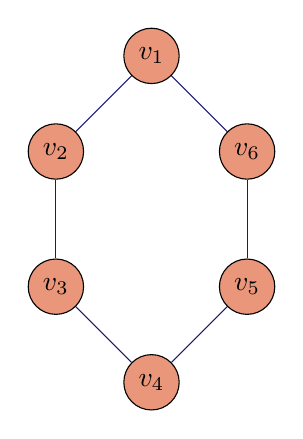
\begin{tikzpicture}
\node[obs, fill=DarkSalmon] (r1) {$v_1$};
\node[obs, below left=of r1, fill=DarkSalmon] (r2) {$v_2$};
\node[obs, below=of r2, fill=DarkSalmon] (r3) {$v_3$};
\node[obs, below right=of r3, fill=DarkSalmon] (r4) {$v_4$};
\node[obs, above right=of r4, fill=DarkSalmon] (r5) {$v_5$};
\node[obs, above=of r5, fill=DarkSalmon] (r6) {$v_6$};
\edge [-, color=MidnightBlue, bend right=30] {r1} {r2} ;
\edge [-, color=MidnightBlue, bend left=30] {r1} {r6} ;
\edge [-, color=MidnightBlue] {r2} {r3} ;
\edge [-, color=MidnightBlue, bend right=30] {r3} {r4} ;
\edge [-, color=MidnightBlue, bend right=30] {r4} {r5} ;
\edge [-, color=MidnightBlue] {r5} {r6} ;
\end{tikzpicture}
%
 \hspace{4cm} 
 %
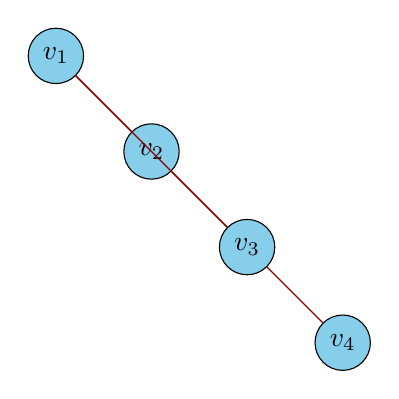
\begin{tikzpicture}
\node[obs, fill=SkyBlue] (r1) {$v_1$};
\node[obs, below right=of r1, fill=SkyBlue] (r2) {$v_2$};
\node[obs, below right=of r2,  fill=SkyBlue] (r3) {$v_3$};
\node[obs, below right=of r3,  fill=SkyBlue] (r4) {$v_4$};
\edge [-, color=DarkRed] {r1} {r2} ;
\edge [-, color=DarkRed, bend right=30] {r1} {r3} ;
\edge [-, color=DarkRed] {r2} {r3} ;
%\edge [-, color=DarkRed, bend left=30] {r2} {r4} ;
\edge [-, color=DarkRed] {r3} {r4} ;
\end{tikzpicture}
\vspace{.5cm}
\caption{Examples of simple undirected graphs. In \textsc{graph A} each node has two neighbors. In \textsc{graph B} node $v_4$ has only a single neighbor while the others each have two neighbors.}
\label{fig:undirected_graphs}
\end{figure}

 An undirected graph $\mathbf{G} = (V,E)$ is simply an ordered pair of sets containing the vertices (also called nodes) and edges of the graph, respectively. In what follows assume that $V$ and $E$ are finite and let $e_{ij} \in E$ denote the element in $E$ that corresponds to the edge connecting the vertices $v_i$ and $v_j$ in $V$. The term {\it undirected} refers to the fact that the edges lack orientation.\footnote{Intuitively, it is helpful to think of the edges of an undirected graph as line segments with no implied direction, whereas the edges in a directed graph can be thought of as arrows.} The {\it neighbors} of node $v_j$ are all nodes $v_i$ such that, for all $i \neq j$ , there is an edge $e_{ij}$. The notation $\partial^{\mathbf{G}}_j$ will be used for the {\it neighborhood} of node $v_j$ in graph  $\mathbf{G}$ and $\partial^\mathbf{G}$ for the set containing the neighborhoods for all nodes in $\mathbf{G}$.\footnote{$ \partial^\mathbf{G}_j = \{v_{i \neq j} \in V \,\vert\, e_{ij} \in E\}$ and $\partial^\mathbf{G} = \{\partial^\mathbf{G}_j \,\vert\, v_j \in V\}$.} For example, in Figure~\ref{fig:undirected_graphs}, $\partial^{\mathbf{A}}_1 = \{v_2, v_6\}$ and $\partial^{\mathbf{B}}_1 = \{v_2, v_3\}$.  For a more comprehensive discussion of undirected graphs in the context of GMRFs see \citeA{rue_gaussian_2005}. 
 

\subsection{GMRFs}
Let $\theta \in \mathbb{R}^D$ have a multivariate normal distribution with probability density function $p(\theta | \mu, \boldsymbol{\Sigma}) = \mathcal{N}_D (\theta | \mu, \boldsymbol{\Sigma})$. The random vector $\theta$ is said to form a GMRF with respect to the graph $\mathbf{G} = (V,E)$ if for each element in $\theta$ there is a corresponding node in $V$, and there is no edge $e_{ij}$ between nodes $v_i$ and $v_j$ \emph{if and only if} $\theta_i$ and $\theta_j$ are conditionally independent given all other elements of $\theta$ \shortcite{rue_gaussian_2005}.\footnote{$v_i \notin \partial^\mathbf{G}_{j} \iff \theta_i \bot \theta_j \mid \theta_{-ij}$}\footnote{This definition is consistent with the definition of Markov random fields in general. The random variables $\theta_1, \dots, \theta_D$ obey the requisite Markov properties describing pairwise, local, and global conditional independencies.} 

The relationship between $G$ and $\theta$ -- the information they provide about each other -- is fully contained in the covariance matrix $\boldsymbol{\Sigma}$, but it is not obvious from the individual elements of $\boldsymbol{\Sigma}$.\footnote{Nothing about the conditional independencies among the elements of $\theta$ can be inferred from the mean vector $\mu$.} It is more useful to instead consider the precision (inverse covariance) matrix $\mathbf{Q}=\boldsymbol{\Sigma}^{-1}$, for which it can be shown that conditional independence between $\theta_i$ and $\theta_j$ (no edge between nodes $v_i$ and $v_j$) always corresponds to a zero in cell $ij$ of the precision matrix, and vice-versa $(\forall i \neq j, \:\: v_i \in \partial_j \iff q_{ij} = 0)$.  For a simple proof see \citeA{rue_gaussian_2005}.\footnote{For intuition, the following interpretations of the elements of a precision matrix may also be helpful to keep in mind. For $i \neq j$ (the off-diagonal), $q_{ij}  = -Cov(\theta_i, \theta_j | \theta_{-ij}) $, the negative (flipped sign) covariance between $\theta_i$ and $\theta_j$ conditional on all $\theta$s except $i$ and $j$.  For $i = j$ (the diagonal),  $q_{ij} = Var(\theta_i | \theta_{-i})$, the variance of $\theta_i$ conditional all the variables except $\theta_i$.}






\section{Bayesian STAR models}
\label{star}

An extension of generalized linear models (GLMs), semiparametric structured additive regression (STAR) models replace the linear predictor with a structured additive predictor of the form
%
\begin{equation*}
\eta =  u'\gamma + \sum_{j} f_j (x_j) =  u'\gamma + f_1(x_1) + \ldots + f_j(x_j) + \ldots + f_J(x_J),
\end{equation*}
%
\noindent which can include nonlinear unknown functions of covariates as well as linear components \shortcite{fahrmeir_bayesian_2001}. 

From the Bayesian perspective, the non-varying parameters $\gamma$ as well as the unknown functions $f_1, \dots, f_J$ are treated as random variables distributed according to priors that we must specify. For an unknown function $f_j$ of a covariate $x_j$ let $\mathbf{f}_j^{eval}$ denote the vector of function evaluations of $f_j$ at each of the $N$ observed values of $x_j$ 

\begin{equation*}
\mathbf{f}_j^{eval} = \left(f_j(x_{1j}), \dots f_j(x_{Nj})\right)'.  
 \end{equation*}
 
\noindent Then $\mathbf{f}_j^{eval}$ is treated as a random vector, which, following \citeA{brezger_generalized_2006}, can conveniently be expressed as the matrix product $\mathbf{M}_j \theta_j$ of a design matrix $\mathbf{M}_j$ and a parameter vector $\theta_j$. GMRF priors for each parameter vector $\theta_j$ take the general form

\begin{equation*}
p(\theta_j | \tau^2_j) 
\propto 
\frac{1}{\left(\tau^2_j\right)^{{\rm rank}(\mathbf{P})/2} }
\exp{\left\{-\frac{1}{2\tau^2_j} \theta_j' \mathbf{P} \theta_j\right\}}
\end{equation*}

\noindent where $\mathbf{P}$ is a penalty matrix whereby we operationalize our prior assumptions about the smoothness of the unknown function $f_j$. 

To provide some intuition, suppose we are interested in learning about an effect with assumed variation over geographic regions.  A simple map with $R$ distinct regions $r_1, r_2, \dots r_R$ can be represented as undirected graph $G$ with vertices $V = \{1, 2, \dots, R\}$ and edges $E$ connecting vertices corresponding to neighboring (or proximate) regions. Assuming some degree of dependence of the quantity of interest across regions, a prior on a parameter vector $\theta = (\theta_1, \dots, \theta_r)$ can be constructed such that the matrix $\mathbf{P}$ has a zero in the $ij$th cell if and only if $\theta_i$ and $\theta_j$ (the parameters corresponding to regions $r_i$ and $r_j$) are assumed to be independent conditional on $\theta_{-ij}$. Then $\theta$ is a GMRF with respect to $G$ with $\boldsymbol{\Sigma}^{-1} = \mathbf{Q} = \mathbf{P}/\tau^2$. 

\subsection{The penalty matrix} 
\label{penalty_matrix}

More specifically, the penalty matrix $\mathbf{P}$ can be constructed as  $\mathbf{P} = \mathbf{D} - \mathbf{A}$, where $\mathbf{A}$ is a symmetric matrix with $a_{ij} = 1$ if temporal or spatial units $i$ and $j$ are considered neighbors (the associated graph $G$ has an edge between nodes $i$ and $j$) and 0 otherwise, and $\mathbf{D}$ is a diagonal matrix such that $\forall i = j, \: d_{ij} = \sum_j a_{ij}$. The matrices $\mathbf{A}$ and $\mathbf{D}$ are commonly referred to as the adjacency and degree matrices because encoded in $\mathbf{A}$ are all neighbor relationships (temporal or spatial) and the (diagonal) elements of $\mathbf{D}$ are equal to the number of neighbors (the degree) of each vertex in the graph $G$. 

To illustrate why this form of $\mathbf{P}$ captures these particular assumptions, consider $N$ measurements of a variable $x$, with each measurement of $x$ made at one of $T$ evenly spaced points in time. For simplicity, but without loss of generality,  assume that $x$ is a unit of time and there is exactly one measurement per time period.  The sequence $(x^{[t]})_{t=1}^T$ then corresponds to a grid of points on a line.  \citeA{fahrmeir_bayesian_2001} suggest several possible choices for a prior on a smooth function $f(x)$, the simplest of which is a first order random walk ($RW_1$) prior.  Under the $RW_1$ prior, the first differences $\Delta_t = f(x^{[t]}) - f(x^{[t-1]})$ are treated as independent and identically distributed standard normal random variables. 

While this formulation of the $RW_1$ prior is {\it directed}, conditioning also on $f(x^{[t+1]})$ -- one step into the future -- forms an undirected $RW_1$, where the neighbors of time $t$ are both $t-1$ and $t+1$.  The associated graph $G$ therefore has vertices $V=\{v_t : t=1,\dots,T\}$, each of which has two neighbors, with the exception of $v_1$ and $v_T$, which have one neighbor. The penalty matrix $\mathbf{P}$ corresponding to the $RW_1$ prior with equally spaced observations is the tridiagonal matrix

\begin{equation*}
\mathbf{P} = 
\begin{bmatrix}
1  	& -1 	& 		& 	& \\
-1  	& 2 	& -1 		& 	& \\
  	& -1 	& \ddots 	& \ddots	& \\
  	&  	& \ddots 	& 2 	& -1\\
  	&  	& 		& -1 	& 1\\
\end{bmatrix}
\end{equation*}

\noindent which can be derived by computing the difference of the appropriate degree and adjacency matrices \shortcite{brezger_generalized_2006}.\footnote{The construction of $\mathbf{P}$ as the matrix difference $\mathbf{D} - \mathbf{A}$ also allows for the estimation of a parameter $\omega \in [0,1]$, which, as a coefficient on $\mathbf{A}$, can be interpreted as representing the strength of spatial or temporal dependence \shortcite{rue_gaussian_2005}. The resulting precision matrix $\mathbf{Q}= (\mathbf{D} - \omega \mathbf{A})/\tau^2$ is the defining feature of the conditional autoregressive (CAR) model.  When $\omega = 1$, and thus $\mathbf{P}= \mathbf{D} - \mathbf{A}$, the model is sometimes referred to as an intrinsic CAR model.
} The $RW_1$  can be extended to an $RW_2$ prior by also considering the measurements $x^{[t-2]}$  and $x^{[t+2]}$ to be neighbors of $x^{[t]}$. 


\subsection{Hyperpriors}
\label{hyperpriors}

To complete the hierarchical model requires also specifying hyperpriors $p(\tau_j^2)$.  Assigning a prior distribution to the variance hyperparameter $\tau_j^2$ allows for the simultaneous estimation of a smoothing function $f_j$ and the amount of smoothness. \citeA{fahrmeir_bayesian_2001} and \citeA{brezger_bayesx:_2005} recommend a weakly informative but proper inverse-gamma prior on $\tau_j^2$. However, in light of concerns about this type of inverse-gamma prior raised by \citeA{gelman_prior_2006}, in this thesis several priors for $\tau^2_j$ are used and compared to check the degree to which the results are sensitive to the choice of prior.


\chapter{Empirical example: Cox and Katz (2007)}
\label{cox_katz}

To demonstrate the benefits of the methods proposed by \citeA{wawro_designing_2014}, we conduct a reanalysis of \citeA{cox_gerrymandering_2007}, a study of bias and responsiveness in congressional roll-call votes in the 46th through 106th US Congresses.\footnote{In the legislative context of Cox and Katz's analysis, bias refers to an advantage for one party in the efficiency with which its votes translate into legislative victories. For example, consider a majority party with only a small advantage in the number of seats its members occupy. If the majority is well-organized and unified it may win a much larger proportion of votes than its slim seat advantage would typically suggest \shortcite{cox_gerrymandering_2007}.} Cox and Katz hypothesize and find evidence of persistent bias towards the majority party during the periods from 1889-1910 and 1961-2000, known as the period of ``czar rule" and the post-packing era, respectively. Using the same data, we find much weaker evidence for bias towards the majority over the time periods in question.\footnote{On the whole, \citeA{cox_gerrymandering_2007} is an excellent paper and covers much more than the single analysis discussed in this thesis. The use of Cox and Katz's analysis here is not intended to single it out for criticism. It simply happens to be a good candidate for testing the approach advocated by Wawro and Katznelson.} 





%Cox and Katz (2007) is a study of bias and responsiveness in the 46th through 106th Congresses. Cox and Katz are predominantly concerned with estimating the parameters $\lambda = \{\lambda_t : t = 46, \dots, 106\}$ representing bias in each $C_t$ (Congress t), which they do by maximum likelihood estimation of grouped logit models with linear predictor
%
%$$ \lambda_t + \rho_t \log{\left(\frac{v_t}{1 - v_t} \right)}, $$
%
%\noindent where $\rho$ is responsiveness and $v$ is average Democratic vote share. They use this strategy to estimate what they call ``a sort of running average" of the bias across time, where they take as their estimate of $\lambda_t$ the average estimate of $\lambda$ over the seven congresses centered at $t$, i.e., the set of congresses $\{C_\tau, t-3 \leq \tau \leq t+3\}$. 
%
%Note that this strategy requires using the data for each Congress up to seven times, which can lead to overly precise parameter estimates. Moreover, the estimation strategy used by Cox and Katz treats each of the seven congresses centered at $t$ as providing {\it equal} information about $\lambda_t$, which is unlikely to be the case. 
%
%Many new possibilities are available to us if we can reformulate their model according to the Bayesian approach advocated above. Let $x = \log{\left(\frac{v_t}{1 - v_t} \right)}$. We use the addititive predictor
%
%$$ \eta = f_1(\lambda) + f_2(x),$$
%
%where the $f_j$ are unknown functions such that the vector of evaluations of $f_j$ can be expressed as the product $\theta_j \mathbf{M}_j$ of a parameter vector $\theta_j$ and a design matrix $\mathbf{M}_j$.  We can then assign a prior for $f_j$ by specifying a suitable $\mathbf{M}_j$ and a (typically partially improper) multivariate normal prior 
%%
%$$ p(\theta_j | \tau_j^2) \propto \exp{\left(-\frac{1}{2\tau_j^2} \theta_j^T \mathbf{P}^{-1} \theta_j \right)}, $$
%
%\noindent where we choose to specify a penalty matrix $\mathbf{P}$ that represents our assumptions of temporal dependence between adjacent Congresses. 
%
% For example, suppose we want to specify a prior that reflects a belief that $\partial_t = \{C_{t-2}, C_{t-1}, C_{t+1}, C_{t + 2} \}$ provides information about $C_t$. We will refer to the elements of $\partial_t$ as the {\it neighbors} of $C_t$. We can use an undirected form of a second order random walk or autoregressive prior to penalize deviations from this hypothesized trend, which corresponds to setting $\mathbf{P} = \mathbf{D} - \mathbf{A}$, where $\mathbf{A}$ is a symmetric matrix with $a_{ij} = 1$ if $C_j \in \partial_i$ and 0 otherwise, and $\mathbf{D}$ is a diagonal matrix such that $\forall i = j, \: d_{ij} = \sum_j a_{ij}$.\footnote{It can be useful to conceptualize the neighbor relations as an undirected graph $G$ with vertices $V= \{C_t, t = 46, \dots, 106\}$ and edges connecting the vertices corresponding to neighboring congresses. The penalty matrix $\mathbf{P}$ then has a zero for each missing edge and the resulting multivariate normal distribution is said to form a Markov random field with respect to $G$. The matrices $\mathbf{A}$ and $\mathbf{D}$ are commonly referred to as the adjacency and degree matrices.}   We then specify a hyperprior $p(\tau^2)$, completing the hierarchical model and enabling the concurrent estimation of the unknown function $f$ and the amount of nonparametric smoothing (Fahrmeir and Lang, 2000). 
% 
% Note that this approach enables us to account for temporal dependence without reusing the data to estimate separate a model for each congress. The Bayesian approach advocated here allows the specification of more intricate temporal relationships that better reflect our assumptions of association across time (and across space in other contexts). For example, a second order random walk prior treats $C_{t-1}$ and $C_{t+1}$ as being more informative than $C_{t-2}$ and $C_{t+2}$ about bias in $C_t$, which seems more reasonable. 

\section{Data}
\label{ckdata}

The data include -- with a few exceptions detailed below -- all roll-call votes in the 
U.S. House of Representatives during the 46th through 106th Congresses, corresponding 
to the period from 1879 to 2001.  Following Cox and Katz, excluded from the analysis are 
any records that meet at least one of the following three conditions: ({\it i}) the majority of 
both parties voted for the same position; ({\it ii}) the purpose of the vote was electing the 
Speaker of the House; ({\it iii}) the vote required a two-thirds majority for passage.

The resulting data consist only of votes that required a simple majority for passage and on 
which the Republican and Democratic parties were in clear opposition.\footnote{A brief 
comment on notation: for greater consistency throughout this paper, this section uses different 
notation than \citeA{cox_gerrymandering_2007}.}

Let $RC_{it}$ denote the result of roll-call vote $i$ in Congress $t$ such that 

\begin{equation*}
RC_{it} =
\begin{cases} 
1, & \text{ if Democratic position wins vote $i$ in Congress $t$,} \\[10pt]
0, & \text{ if Republican position wins vote $i$ in Congress $t$.}
\end{cases}
\end{equation*}
~\\[-12pt]

%\noindent Here, the Democratic position refers to the outcome preferred by the majority of Democrats.  The definition is analogous for the Republican position.

%The outcomes of interest are the number of wins ($w_t^{DEM}$) and proportion of wins ($\pi_t^{DEM}$) for the Democratic position in each Congress $t$
%
%$$ w_t^{DEM} = \sum_{i=1}^{n_t} RC_{it}, \qquad \pi_t^{DEM} = w_t^{DEM} / n_t.\footnote{The superscript {\it MAJ} (e.g. $y_t$) will be used later in the thesis as a general way of referring to the majority party in a specific time period. While the data is organized and more naturally described in terms of $w_t^{DEM}$ and $w_t^{REP}$ (which is just $n_t-w_t^{DEM}$), the proposed statistical model is more straightforward to implement in terms of $w_t^{MAJ.}$}$$
%
%Here $n_t$ is the number of roll-call votes in Congress $t$, which ranges from a minimum of 33 votes in the 70th Congress (1927-1929) to a maximum of 836 votes in the 104th Congress (1995-1997). The median number is 143 votes.  
%
%
%The sole predictor of interest is $v^{RATIO}$, the ratio of the average vote share earned by the Democratic position to the average vote share earned by the Republican position in each Congress.  For each Congress the average is taken over all roll-call votes.  For vote $i$ in Congress $t$, let $\pi_{it}^{DEM}$ be the proportion of representatives who cast their vote in favor of the Democratic position.  Then the mean vote shares for the Democratic and Republican positions in Congress t is
%
%{\singlespacing
%$$v_t^{DEM} = \frac{1}{n_t} \sum_{i=1}^{n_t} \pi_{it}^{DEM}, \qquad v_t^{REP} = 1 - v_t^{DEM}$$
%}
%%
%\noindent and the ratio of Democratic to Republican vote shares is simply $v_t^{RATIO} = v_t^{DEM} / v_t^{REP}$. Figure~\ref{fig:log_vratio_vs_ptdem} shows $\log{(v^{RATIO} )}$ plotted against $\pi^{DEM}$. The shape of the curve is similar to the standard seats-votes curve used in analyses of bias and responsiveness in electoral contexts. The curve is analogous in the legislative context of Cox and Katz's example, although we are not concerned with seat shares in a given Congress but rather roll-call vote shares ($\pi_t^{DEM}$ and $\pi_t^{REP}$). This is discussed further in the Methods section. 
%
%The trends of $\log{(v^{RATIO} )}$ and $\pi^{DEM}$ over time are shown in the visual summary of the data set in Figure~\ref{fig:data_summary}.
%
%%FIGURE
%\begin{figure}
%\centering
%	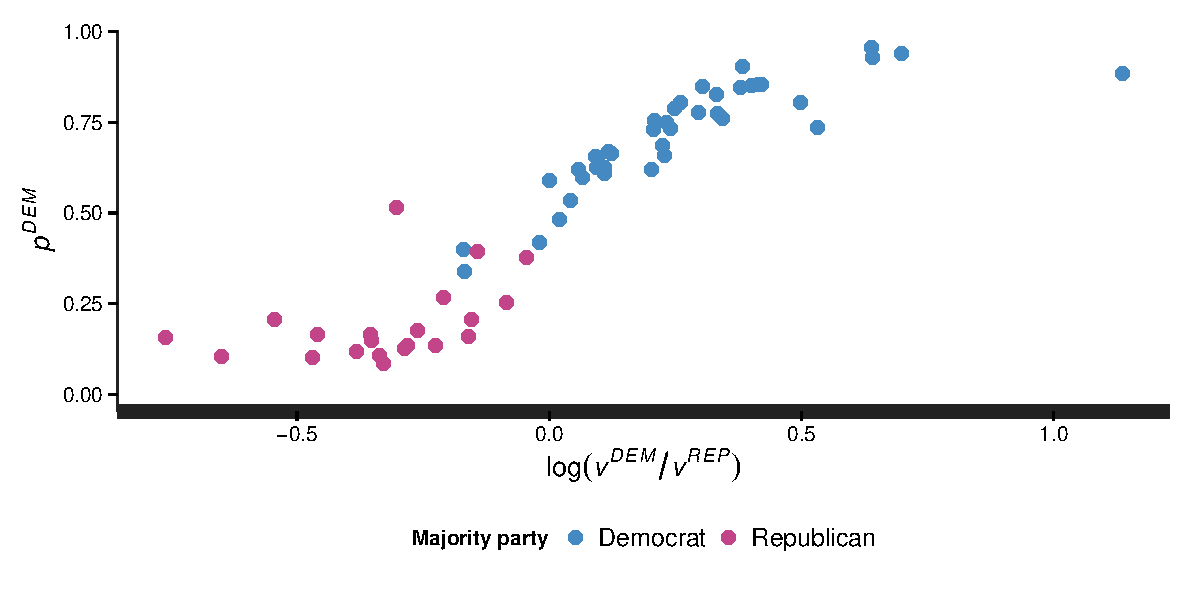
\includegraphics[scale=0.75]{sections/figs/logvratio_vs_pdem}
%\caption{$\log{(v^{RATIO} )}$  vs. $\pi^{DEM}$}
%\label{fig:log_vratio_vs_ptdem}
%\end{figure}
%%
%



\noindent The outcomes of interest are the number of wins $y_t$ and proportion of wins 
$\pi_t$ for the majority party position in each Congress $t$,

\begin{equation*}
y_t =
\begin{cases} \sum_{i=1}^{n_t} RC_{it}, & \text{ if Democrats hold majority}, \\[10pt]
n_t - \sum_{i=1}^{n_t} RC_{it}, & \text{ if Republicans hold majority,} \\
\end{cases}
\end{equation*}
~\\[-12pt]
 
\noindent and $\pi_t = y_t / n_t$. Here $n_t$ denotes the number of roll-call votes in 
Congress $t$.\footnote{The value of $n$ ranges from a minimum of 33 votes in the 
70th Congress (1927-1929) to a maximum of 836 votes in the 104th Congress (1995-1997). 
The median number is 143 votes. See also Figure~\ref{fig:data_summary} 
(p. \pageref{fig:data_summary}).} 


The sole predictor is the ratio of the average vote share earned by the majority party position 
to the average vote share earned by the minority party position in each Congress.  (For each 
Congress the average is taken over all roll-call votes.)  For vote $i$ in Congress $t$, let 
$p_{it}^{DEM}$ be the proportion of representatives who cast their vote in favor of the Democratic 
position.  Then the mean vote shares for the Democratic and Republican positions in Congress t are

\begin{equation*}
v_t^{DEM} = n_t^{-1} \sum_{i=1}^{n_t} p_{it}^{DEM}, \qquad v_t^{REP} = 1 - v_t^{DEM},
\end{equation*}

\noindent and the ratio of Democratic to Republican vote shares is simply $v_t^{DEM} / v_t^{REP}$. The notation $v_t^{RATIO}$ will be used as shorthand for the ratio $v_t^{MAJ} / v_t^{MIN}$, that is 

\begin{equation*}
v^{RATIO} = 
\begin{cases} 
v^{DEM} / v^{REP}, & \text{ if Democrats hold the majority,} \\[10pt]
v^{REP} / v^{DEM}, & \text{ if Republicans hold the majority.} \\
\end{cases}
\end{equation*}
~\\[-12pt]


%FIGURE
\begin{figure}
\centering
	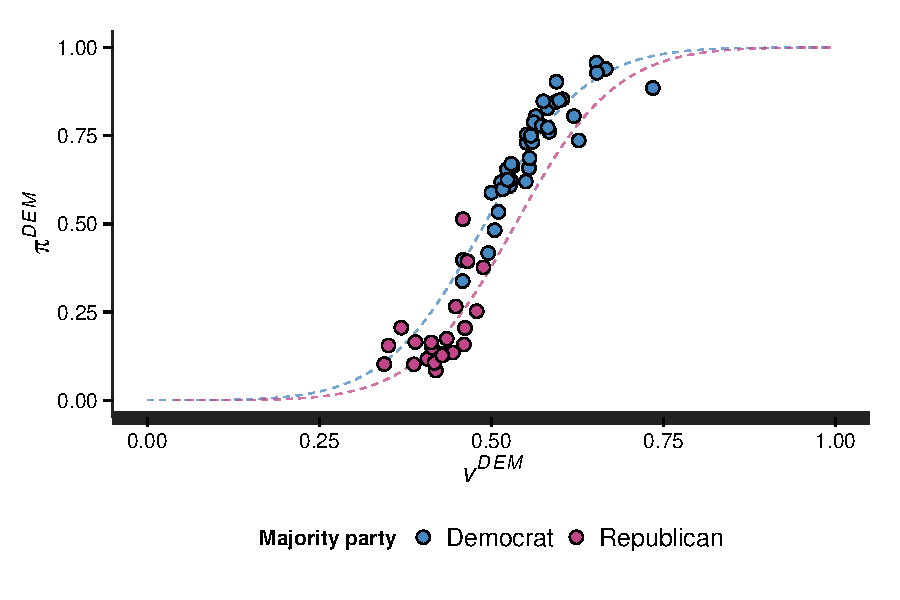
\includegraphics[scale=0.75]{sections/figs/vdem_vs_pdem}
\caption{Average Democratic vote-share $(v^{\it DEM})$ in Congress $t$ vs. Total proportion of votes won $(\pi^{DEM})$ in Congress $t$. Each point represents a Congress. Dashed lines show estimated seats-votes curves. (See also Figure~2 in \protect\citeA{cox_gerrymandering_2007}.)}
\label{fig:log_vratio_vs_ptdem}
\end{figure}


Figure~\ref{fig:log_vratio_vs_ptdem} shows $v^{\it DEM}$ plotted against $\pi^{DEM}$. The shape of the curve is suggestive of the standard seats-votes curve  

\begin{equation*}
 \frac{s}{1-s} = \exp{(\lambda)}\left(\frac{v}{1-v}\right)^\rho 
\end{equation*}

\noindent used in analyses of bias and responsiveness in electoral contexts. The curve is 
analogous in the legislative context of Cox and Katz's example but for roll-call vote shares 
$\pi$ rather than seat shares $s$. This is discussed further in section \ref{subsection_methods}
 in relation to the statistical model.\footnote{See also Appendix~\ref{AppendixB} for visual 
 examples of seats-votes curves.}

The trends of $\log{(v^{\it RATIO})}$ and $\pi^{MAJ}$ over time are shown in the visual summary 
of the dataset in Figure~\ref{fig:data_summary} (p.~\pageref{fig:data_summary}). \\[10pt]


%FIGURE
\begin{figure}[p]
\centering
	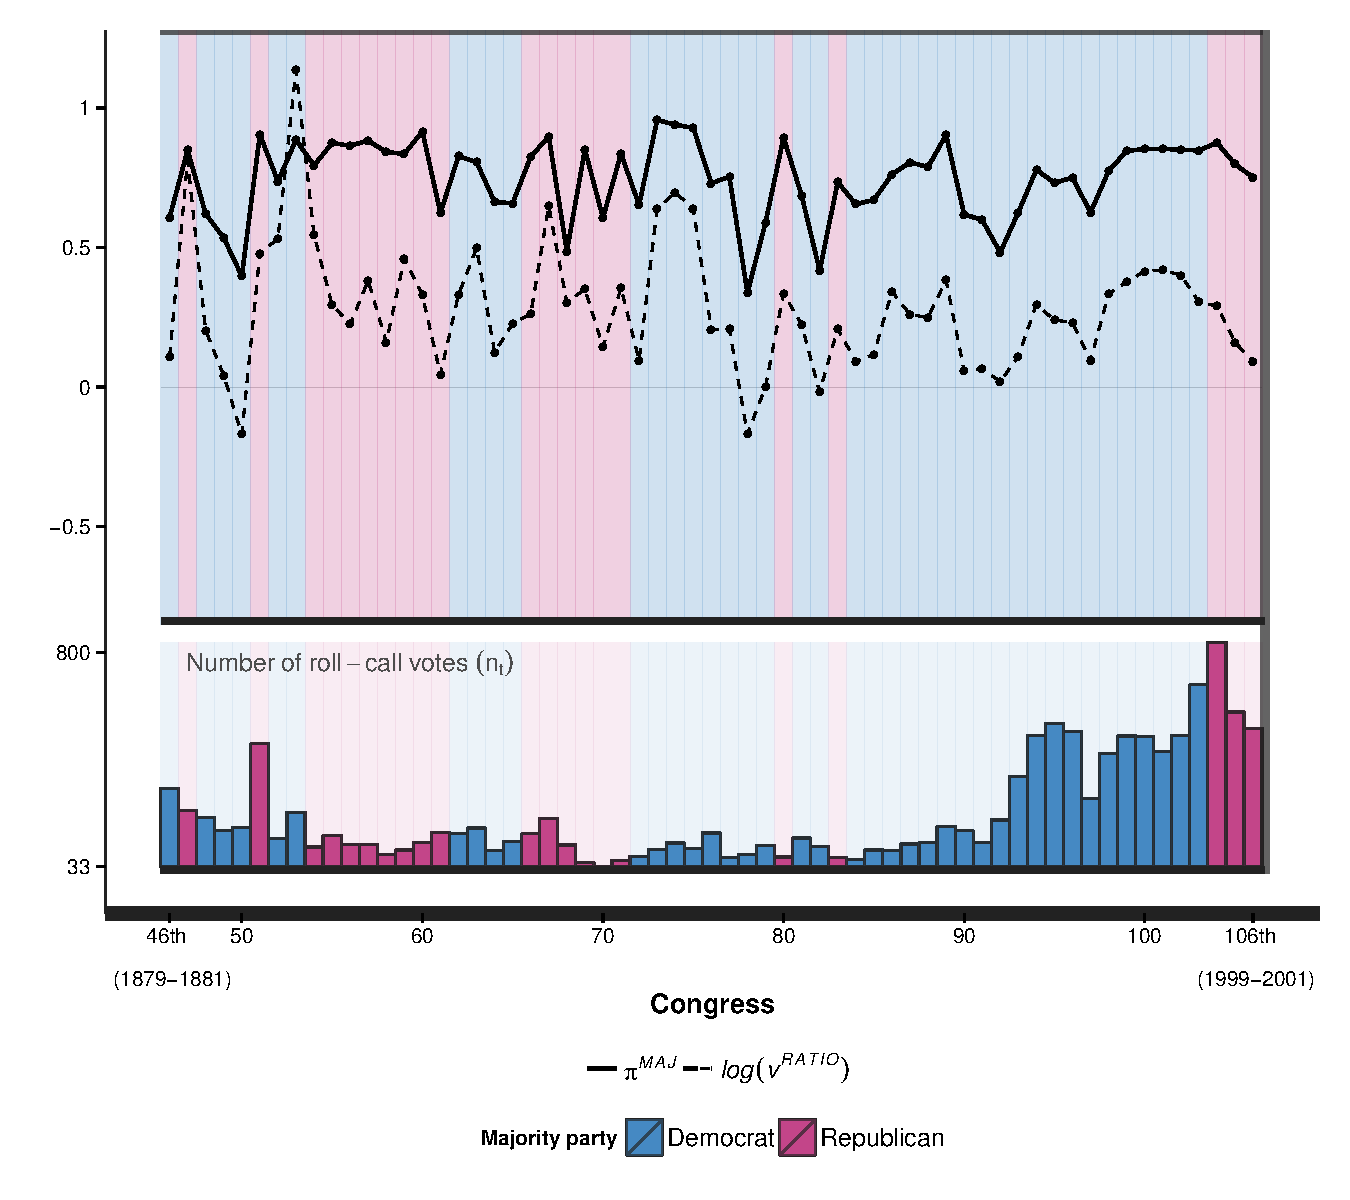
\includegraphics[scale=0.75]{sections/figs/vis_summary}
\caption{Visual summary of the data. The trends of $\log{(v^{\it RATIO} )}$ and $\pi^{MAJ}$ by 
Congress are plotted on top, with the number of roll-call votes per Congress below. Background 
shading is used to differentiate between Democratic and Republican majorities.}
\label{fig:data_summary}
\end{figure}
%

%One method of identifying bias toward or against the majority party is to estimate $E[p_t |v_t^{MAJ}=0.5]$, the proportion of majority party victories conditional on equal vote share, and compare the estimate to $0.5$, the expected proportion of majority party victories in the absence of bias.  There are many close votes in the data -- that is, votes where $v_t^{MAJ} \approx 0$ -- which can be used to estimate $E[p_t |v_t^{MAJ}=0.5]$.  Figure 2, below, shows the proportion of majority party victories under four different definitions of a close votes corresponding to margins of victory of 0.125\%, 0.25\%, 0.5\%, and 1.0\%. 
%
%\vskip1cm
%FIGURE
%\vskip1cm


\section{Statistical and computational methods}
\label{ck_stats}

\subsection{Description of statistical model}
\label{subsection_methods}

\subsubsection{Cox and Katz's analysis}

\citeA{cox_gerrymandering_2007} propose two methods for checking their hypothesis 
of bias towards the majority party during the czar rule and post-packing eras. One strategy 
is to estimate separate models for four historical time periods of interest. 
\citeA{goodrich_designing_2012} advises that this ``imposes a particular periodization scheme 
that, while consistent with received wisdom, may or may not be the correct one" (p. 16). 

Cox and Katz's second approach is more promising in that it allows for greater parameter 
heterogeneity and makes fewer a priori assumptions about the underlying data generating 
process. It is worth noting that making assumptions about the data generating process is in 
general not only unavoidable but also extremely important. The problem with the assumptions 
required for Cox and Katz's first method is not that they are implausible, but rather that 
periodization schemes per se are convenient abstractions that, in the context of quantitative 
historical analysis, can enforce a theoretically motivated but not empirically justified structure 
that should be learned rather than imposed. However, as demonstrated below, there are also 
issues with Cox and Katz's second design that can be overcome by following the recommendations 
in \citeA{wawro_designing_2014}. 

Let $C$ denote the number of unique Congresses (time periods) in the data. 
The analysis conducted by Cox and Katz centers on estimating the parameters  
$\lambda = (\lambda_t : t = 1, \dots, C)$ representing bias (on the logit scale) toward 
the majority party in each Congress $t$. They do this by maximum likelihood estimation 
of grouped logit models with linear predictor $ \lambda_t + \rho_t \log{\left(v_t^{Ratio} \right)}$. 

The estimation of $\lambda$ and $\rho$ by grouped logit models follows naturally from 
solving the seats-votes equation for the average seat share. In the legislative context of 
Cox and Katz's example this means solving for the expected roll-call win share for the 
majority as

\begin{equation*}
  E(\pi_t)  = \left(1 + \exp{\left\{- \lambda_t - \rho_t \log{\left( v_t^{Ratio}  \right)}\right\}}\right)^{-1},
\end{equation*}
%
\noindent which is the familiar logistic function. 

Cox and Katz's strategy is to estimate what they call ``a sort of running average" of bias 
across time (p. 116). To do this they take as their estimate of $\lambda_t$ the average 
estimate of $\lambda$ over the seven congresses centered at $t$. However, this 
approach to modeling temporal dependence in $\lambda$ requires reusing the data 
to estimate models for each Congress -- the observations for each Congress are used 
up to seven times.  \citeA{goodrich_designing_2012} points out that such recycling of 
data can lead to overly precise parameter estimates (this point is discussed further and 
corroborated visually in \ref{results}). 

Although Cox and Katz do not address this potential for exaggerated precision, they do 
call attention to another  concern. To obtain reasonable estimates, their method requires 
nontrivial variation in average vote share between the seven Congresses centered at 
$t$.\footnote{Technically there will be fewer than seven Congresses for $t < 4$ as well as 
$t > C- 3$, but the idea is the same regardless of the exact number.}

\subsubsection{Alternative analysis with Bayesian STAR model}

The alternative analysis presented below overcomes both of these concerns by employing 
a hierarchical Bayesian framework which takes advantage of partial pooling. Following Cox 
and Katz, a BetaBinomial likelihood is used, however the linear predictor is replaced by the 
structured additive predictor $\eta$. 

The ${\rm Beta\text{-}Binomial}(n,\alpha,\beta)$ distribution can be thought of as a compound 
distribution resulting from a ${\rm Binomial}(n,p)$ distribution where $p \sim {\rm Beta}(\alpha,\beta)$. 
Rather than assuming a fixed probability of a majority party roll-call victory -- in which case a simple 
binomial model would suffice -- the beta-binomial distribution treats the underlying probability $p$ 
as a random variable. The parameters $\alpha > 0$ and $\beta > 0$ govern the shape of the beta 
distribution, however it is both more intuitive and computationally attractive to reparameterize in terms 
of the mean $\theta = \alpha / (\alpha + \beta)$, which requires introducing an auxiliary parameter 
$\phi = \alpha + \beta$. 

This parameterization allows for modeling ${\rm logit}(\theta)$ by the semi-parametric structured 
additive predictor $\eta$ of the STAR model, which can be written in vector/matrix notation 
as 

\begin{equation*}
 \eta = f_\lambda(t) +  f_\rho(\log{(v^{Ratio})}). 
\end{equation*}

\noindent As discussed in \ref{star}, the vectors of function evaluations are 
expressed as the products 

\begin{equation*}
\mathbf{f}^{eval}_\lambda = \mtrx{M}_\lambda \lambda, 
\qquad 
\mathbf{f}^{eval}_\rho =  \mtrx{M}_\rho \rho, 
\end{equation*}
%
\noindent of the parameter vectors $\lambda \in \mathbb{R}^C$ and $\rho \in \mathbb{R}^C$ 
premultiplied by the $N \times C$ design matrices  $\mathbf{M}_\lambda$ and  $\mathbf{M}_\rho$ 
($N$ is the number of observations). The matrices $\mathbf{M}_\lambda$ and $\mathbf{M}_\rho$ 
are identical in structure but not content. The elements of $\mathbf{M}_\lambda$ are zeros and ones 
indicating the Congress to which each observation pertains. For $\mathbf{M}_\rho$ each element is 
either a zero or the appropriate value of $\log{(v^{Ratio})}$. 

% Discuss challenges with sparse matrices? Either here or in the lit review section

Priors for $f_{\lambda}$ and $f_{\rho}$ are expressed as distributions over the random 
vectors $\lambda$ and $\rho$ as 

\begin{equation*}
p(\lambda | \tau_\lambda^2, \bar{\lambda}) 
\propto 
\exp{\left\{-\frac{1}{2\tau_\lambda^2} \: \left(\lambda - \bar{\lambda}\right)^\intercal  \mtrx{P}   
\left(\lambda - \bar{\lambda}\right) \right\}} 
\propto 
\mathcal{N} (\lambda | \bar{\lambda}, \mtrx{Q}_\lambda^{-1}), 
\end{equation*}
\begin{equation*}
p(\rho | \tau_\rho^2, \bar{\rho}) 
\propto 
\exp{\left\{-\frac{1}{2\tau_\rho^2} \: \left(\rho - \bar{\rho}\right)^\intercal  \mtrx{P} 
\left(\rho-\bar{\rho}\right) \right\}} 
\propto 
\mathcal{N} (\rho | \bar{\rho}, \mtrx{Q}_\rho^{-1}), 
\end{equation*}

\noindent where $\mathbf{P}$ is the penalty matrix.

To model temporal dependence such that the neighbors of Congress $t$ also provide 
information about the values of the parameters of interest at time $t$, the undirected 
random walk prior discussed in \ref{penalty_matrix} is used. Using the notation 
introduced in \ref{undirected_graphs} we can define adjacency by specifying the 
neighborhoods for all Congresses (time periods) $t = 1, \dots, C$

\begin{equation*}
\partial^\mathbf{G}_t = \left\{C_s : \left| s - t \right| \leq \kappa \right\},
\end{equation*}

\noindent where $\kappa \leq C$ is a positive integer and $\mathbf{G}$ is the undirected graph 
with nodes $V = \{\nu_1, \dots, \nu_C\}$ and the edges implied by $\partial^\mathbf{G}$ 
(see Figure~\ref{fig:rw_undirected_graphs}). The results presented in section~\ref{results} use 
the first order undirected random walk prior for $f_\lambda$ and $f_\rho$, which applies smoothing 
while allowing for slightly more abrupt shifts in parameter values between Congresses than the 
$RW_2$ prior.\footnote{As mentioned in \ref{hyperpriors}, several priors for $\tau^2_\lambda$ 
and $\tau^2_\rho$ were considered including inverse-gamma \shortcite{fahrmeir_bayesian_2001} 
and half-Cauchy \shortcite{gelman_prior_2006}, as well as half-normal. Parameter estimates were 
not sensitive to the choice of prior. For computational reasons (nicer tail behavior) half-normal priors 
are used for the final model presented below.}
 


\begin{figure}[htb]
\centering

\vspace{2cm}

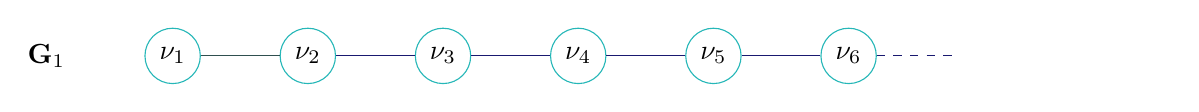
\begin{tikzpicture}
\node[const] (name) {$\mathbf{G}_1$} ;
\node[obs, right=of name,  color=BlueGreen,  fill=white, text=black] (r1) {$\nu_{1}$};
\node[obs, right=of r1, color=BlueGreen,  fill=white, text=black] (r2) {$\nu_{2}$};
\node[obs, right=of r2, color=BlueGreen,  fill=white, text=black] (r3) {$\nu_{3}$};
\node[obs, right=of r3, color=BlueGreen,  fill=white, text=black] (r4) {$\nu_{4}$};
\node[obs, right=of r4, color=BlueGreen,  fill=white, text=black] (r5) {$\nu_{5}$};
\node[obs, right=of r5, color=BlueGreen,  fill=white, text=black] (r6) {$\nu_{6}$};
\node[const, right=of r6] (dots1) {$\hspace{.33cm}$};
\node[const, right=of dots1] (dots2) {$\hspace{.33cm}$};
\node[const, right=of dots2] (dots3) {$$};
\edge [-, color=DarkSlateGray, bend left = 5] {r1} {r2} ;
\edge [-, color=MidnightBlue, bend right = 5] {r2} {r3} ;
\edge [-, color=MidnightBlue, bend left = 5] {r3} {r4} ;
\edge [-, color=MidnightBlue, bend right = 5] {r4} {r5} ;
\edge [-, color=MidnightBlue, bend left = 5] {r5} {r6} ;
\edge [dashed, -, color=MidnightBlue, bend right = 5] {r6} {dots1} ;
\end{tikzpicture}
%
 \hspace{4cm} 
 %
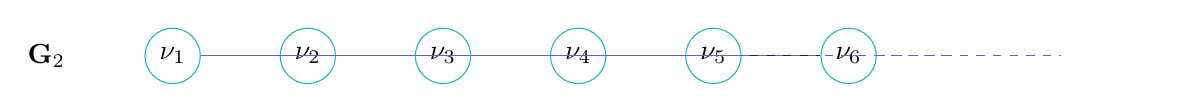
\begin{tikzpicture}
\node[const] (name) {$\mathbf{G}_2$} ;
\node[obs, right=of name,  color=BlueGreen,  fill=white, text=black] (r1) {$\nu_{1}$};
\node[obs, right=of r1, color=BlueGreen,  fill=white, text=black] (r2) {$\nu_{2}$};
\node[obs, right=of r2, color=BlueGreen,  fill=white, text=black] (r3) {$\nu_{3}$};
\node[obs, right=of r3, color=BlueGreen,  fill=white, text=black] (r4) {$\nu_{4}$};
\node[obs, right=of r4, color=BlueGreen,  fill=white, text=black] (r5) {$\nu_{5}$};
\node[obs, right=of r5, color=BlueGreen,  fill=white, text=black] (r6) {$\nu_{6}$};
\node[const, right=of r6] (dots1) {$\hspace{.33cm}$};
\node[const, right=of dots1] (dots2) {$\hspace{.33cm}$};
\node[const, right=of dots2] (dots3) {$$};
\edge [-, color=MidnightBlue, bend left = 5] {r1} {r2} ;
\edge [-, color=SlateBlue, bend left=30] {r1} {r3} ;
\edge [-, color=MidnightBlue, bend right = 5] {r2} {r3} ;
\edge [-, color=SlateBlue, bend right=30] {r2} {r4} ;
\edge [-, color=MidnightBlue, bend left = 5] {r3} {r4} ;
\edge [-, color=SlateBlue, bend left=30] {r3} {r5} ;
\edge [-, color=MidnightBlue, bend right = 5] {r4} {r5} ;
\edge [-, color=SlateBlue, bend right=30] {r4} {r6} ;
\edge [-, color=MidnightBlue, bend left = 5] {r5} {r6} ;
\edge [dashed, -, color=SlateBlue, bend left=30] {r5} {dots1} ;
\edge [dashed, -, color=MidnightBlue, bend right = 5] {r6} {dots1} ;
\edge [dashed, -, color=SlateBlue, bend right=30] {r6} {dots2} 
\end{tikzpicture}
%
 \hspace{4cm} 
 %
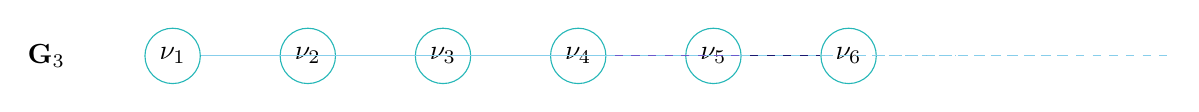
\begin{tikzpicture}
\node[const] (name) {$\mathbf{G}_3$} ;
\node[obs, right=of name,  color=BlueGreen,  fill=white, text=black] (r1) {$\nu_{1}$};
\node[obs, right=of r1, color=BlueGreen,  fill=white, text=black] (r2) {$\nu_{2}$};
\node[obs, right=of r2, color=BlueGreen,  fill=white, text=black] (r3) {$\nu_{3}$};
\node[obs, right=of r3, color=BlueGreen,  fill=white, text=black] (r4) {$\nu_{4}$};
\node[obs, right=of r4, color=BlueGreen,  fill=white, text=black] (r5) {$\nu_{5}$};
\node[obs, right=of r5, color=BlueGreen,  fill=white, text=black] (r6) {$\nu_{6}$};
\node[const, right=of r6] (dots1) {$\hspace{.33cm}$};
\node[const, right=of dots1] (dots2) {$\hspace{.33cm}$};
\node[const, right=of dots2] (dots3) {$$};
\edge [-, color=MidnightBlue, bend left = 5] {r1} {r2} ;
\edge [-, color=SlateBlue, bend left=30] {r1} {r3} ;
\edge [-, color=SkyBlue, bend left=45] {r1} {r4} ;
\edge [-, color=MidnightBlue, bend right = 5] {r2} {r3} ;
\edge [-, color=SlateBlue, bend right=30] {r2} {r4} ;
\edge [-, color=SkyBlue, bend right=45] {r2} {r5} ;
\edge [-, color=MidnightBlue, bend left = 5] {r3} {r4} ;
\edge [-, color=SlateBlue, bend left=30] {r3} {r5} ;
\edge [-, color=SkyBlue, bend left=45] {r3} {r6} ;
\edge [-, color=MidnightBlue, bend right = 5] {r4} {r5} ;
\edge [-, color=SlateBlue, bend right=30] {r4} {r6} ;
\edge [dashed, -, color=SkyBlue, bend right=45] {r4} {dots1} ;
\edge [-, color=MidnightBlue, bend left = 5] {r5} {r6} ;
\edge [dashed, -, color=SlateBlue, bend left=30] {r5} {dots1} ;
\edge [dashed, -, color=SkyBlue, bend left=45] {r5} {dots2} ;
\edge [dashed, -, color=MidnightBlue, bend right = 5] {r6} {dots1} ;
\edge [dashed, -, color=SlateBlue, bend right=30] {r6} {dots2} 
\edge [dashed, -, color=SkyBlue, bend right=45] {r6} {dots3} 
\end{tikzpicture}
\vspace{.25cm}

\caption{The undirected graphs corresponding to $\kappa = 1$, $\kappa = 2$ and $\kappa = 3$. 
Each node represents a Congress. The dashed lines indicate that only part of the graph is shown 
due to space constraints.}
\label{fig:rw_undirected_graphs}
\end{figure}


%As alluded to above, modeling the temporal dependence between Congresses is accomplished via the choice of penalty matrix $\mathbf{P}$. To model temporal dependence such that the set of Congresses $\partial_t = \{C_{t-2}, C_{t-1}, C_{t+1}, C_{t + 2} \}$ provides information about $C_t$, an undirected form of a second order random walk or autoregressive prior is used to penalize deviations from this hypothesized trend. This corresponds to setting $\mathbf{P} = \mathbf{D} - \mathbf{A}$, where $\mathbf{A}$ is a symmetric matrix with $a_{ij} = 1$ if $C_j \in \partial_i$ and 0 otherwise, and $\mathbf{D}$ is a diagonal matrix such that $\forall i = j, \: d_{ij} = \sum_j a_{ij}$. It can be useful to conceptualize the neighbor relations described by each set $\partial_t$ as an undirected graph $G$ with vertices $V=\{C_t: t=46,\dots,106\}$ and edges connecting the vertices corresponding to neighboring Congresses.\footnote{Note that here the term ``neighbor" is not reserved only for adjacent Congresses, but rather any Congress in $\partial_t$ is considered a neighbor of Congress $t$.} The penalty matrix $\mathbf{P}$ then has a zero for each missing edge and the resulting multivariate normal distribution is a GMRF with respect to $G$.
%
%The matrices $\mathbf{A}$ and $\mathbf{D}$ are commonly referred to as the adjacency and degree matrices because encoded in $\mathbf{A}$ are all neighbor relationships (in this case a temporal relationship between Congresses) and the diagonal elements of $\mathbf{D}$ are the number of neighbors (the degree) of each vertex.
%
%To illustrate why this form of $\mathbf{P}$ captures these particular assumptions, consider $N$ measurements of a variable $x$, with each measurement made at one of $T$ evenly spaced points in time. For simplicity assume $N=T$ and that unit of $x$ is a unit of time.  The sequence of equally spaced time measurements $(x^{[t]})_{t=1}^T$ corresponds to a grid of points on a line.  Fahrmeir & Lang (2001) suggest several possible choices for a prior on a smooth function $f(x)$, the simplest of which is a first order random walk ($RW_1$) prior.  Under the $RW_1$ prior, the first differences
%
%$$\Delta_t = f(x^{[t]}) - f(x^{[t-1]})$$
%
%are treated as independent and identically distributed standard normal random variables. 
%
%While this formulation of the $RW_1$ prior is {\it directed}, conditioning also on $f(x^{[t+1]})$ -- one step into the future -- forms an undirected $RW_1$, where the neighbors of time $t$ are both $t-1$ and $t+1$.  The associated graph $G$ therefore has vertices $V=\{\nu_t : t=1,\dots,T\}$, each of which has two neighbors, with the exception of $\nu_1$ and $\nu_T$, which have one neighbor. The penalty matrix $\mathbf{P}$ corresponding to the $RW_1$ prior with equally with equally spaced observations is the tridiagonal matrix
%
%$$ \mathbf{P} = \mathbf{D} - \mathbf{A} =  \begin{bmatrix}
%1  	& -1 	& 		& 	& \\
%-1  	& 2 	& -1 		& 	& \\
%  	& -1 	& \ddots 	& \ddots	& \\
%  	&  	& \ddots 	& 2 	& -1\\
%  	&  	& 		& -1 	& 1\\
%\end{bmatrix}
%.
%$$
%
%The $RW_2$ prior used in this thesis is simply an extension of the $RW_1$ to the case where, in addition to $x^{[t-1]}$  and $x^{[t+1]}$, the measurements $x^{[t-2]}$  and $x^{[t+2]}$ are also considered neighbors of $x^{[t]}$. The construction of $\mathbf{P}$ as the matrix difference $\mathbf{D} - \mathbf{A}$ also allows the estimation of an optional scalar parameter $\gamma \in [0,1]$, which, as a coefficient on $\mathbf{A}$, can be interpreted as representing the strength of dependence (Rue and Held, 2005).\footnote{The resulting precision matrix $\mathbf{Q}= (\mathbf{D}- \gamma \mathbf{A})/\tau^2$ is the defining feature of the conditional autoregressive (CAR) model.  When $\gamma$ is fixed at 1, and thus $\mathbf{P}= \mathbf{D} - \mathbf{A}$, it is known as the intrinsic conditional autoregressive (ICAR) model.} In the results section it will be demonstrated that the degree to which the proposed model fits the data depends (slightly but non-negligibly) on the inclusion of $\gamma$. 



 \subsection{Estimation using Stan}
 \label{stan_intro}

For notational convenience, let $x$ represent the observed $n$ (number of roll-call votes) 
and $v^{Ratio}$ (ratio of majority to minority average vote-share).  And let 
$\psi = \big((\tau^2_\lambda, \bar{\lambda}), (\tau^2_\rho, \bar{\rho}), \phi \big)$ denote 
the hyperparameters of the model, and $\bm{f}$ the unknown functions  $f_\lambda$ and 
$f_\rho$. The joint posterior distribution for $(\bm{f}, \psi)$ given the data $(y, x)$ can then 
be more concisely expressed as 

\begin{align*}
p(\bm{f}, \psi | y, x) 
&\propto p(\bm{f}, \psi)  L(y | x, \bm{f}, \psi)  \\
&=p(\psi)  p(\bm{f} | \psi)   \prod_{n=1}^N L(y_n | \eta_n, x_n), 
\end{align*}

\noindent where the second line follows from assumptions of independence and conditional 
independence.\footnote{In particular it is assumed that hyperparameters are mutually independent 
in their priors, $p(f_\lambda | \tau^2_\lambda, \bar{\lambda})$ and $p(f_\rho | \tau^2_\rho, \bar{\rho})$ 
are conditionally independent, and the observations are independent conditional on parameters 
and $x$.}
%\footnote{The absence of the previously mentioned parameters $\alpha$, $\beta$, and $\theta$ from the expression for the posterior distribution is due to the fact that their values are determined by the other parameters.} 

Estimation is performed by Markov chain Monte Carlo (MCMC) approximation and implemented in 
RStan, the R interface to the probabilistic programming language and C++ library Stan 
\shortcite{rstan_software:2015}. Although other existing software including BayesX, JAGS, and 
OpenBugs can sometimes be used to fit similar models by MCMC, each has important limitations 
that Stan overcomes. Several of the many advantages to using Stan are discussed in the next section. 
Since there are few published examples of fitting similar models in Stan, the next section is 
written in the style of a technical vignette, introducing Stan and describing how the model is coded 
and estimated. 

\subsubsection{Brief introduction to Stan}

\citeA{wawro_designing_2014} uses software called BayesX \shortcite{bayesx_software}, which 
is appropriate and  efficient for certain models, but offers limited flexibility in the choice of priors, 
likelihoods, and link functions. To make the recommendations of Wawro and Katznelson more widely 
applicable will require software with greater versatility. \citeA{goodrich_designing_2012} advocates 
using Stan, which can fit a more diverse range of models than is currently possible with BayesX 
and other software packages, and allows for analyses in the spirit of \citeA{wawro_designing_2014} 
to be extended beyond the confines of their particular examples.  

Stan is a probabilistic modeling language, MCMC sampler, and optimizer. The particular MCMC 
algorithm implemented in Stan is a variant of Hamiltonian Monte Carlo (HMC) called the No-U-Turn 
Sampler (NUTS) \shortcite{hoffman_2012}. Borrowing from physics the concepts and mathematics 
behind Hamiltonian dynamics, HMC treats the vector of unknown parameters as the position of a 
particle. In Hamiltonian dynamics, momentum and position change continuously over time, with the 
gradient of the particle's potential energy function --  which corresponds to the negative log posterior 
-- responsible for changes in momentum, and momentum governing changes in position. Stan works 
by simulating a discretization of this process, making necessary corrections to satisfy the detailed 
balance equations (that is, to ensure the resulting Markov chains are reversible).\footnote{Reversibility 
of the Markov chain is important because every reversible Markov chain has a stationary distribution 
(i.e. reversibility is a sufficient, but not necessary condition). Intuitively, reversibility means that for 
$x$ and $x^\prime$ generated from the target density, the probability of the Markov chain 
transitioning from state $x$ to $x^\prime$ is the same as from $x'$ to $x$.}  

Several characteristics of HMC, and in particular Stan's implementation of HMC, make it a more 
appealing choice than traditional Metropolis-Hastings (M-H) and Gibbs samplers, especially for 
complex models with a large number of parameters to estimate \shortcite{hoffman_2012, stan_development_team_stan_2015}. Both M-H and Gibbs samplers suffer from random walk behavior 
that leads to inefficient exploration of the parameter space. M-H algorithms in particular also place the 
burden of tuning the sampler on the user. Gibbs samplers typically involve less tuning, but require 
specifying full conditional distributions for all parameters. Except in a limited number of cases, full 
conditionals are difficult or impossible to derive, which results in conjugate priors being used when 
other priors might be more believable or preferable for other reasons. 

Stan is designed to overcome each of these concerns. The random walk behavior that plagues both 
Gibbs and M-H is largely avoided because HMC uses gradient information to find posterior modes 
much more efficiently, thus greatly reducing the number of iterations required to obtain a sufficient 
effective posterior sample size \shortcite{hoffman_2012}.\footnote{Stan uses reverse-mode automatic
differentiation.}  Although the theory behind HMC does not obviate the need for the user to specify 
tuning parameters, Stan's NUTS-based adaptation algorithm attempts to learn the optimal values 
of all such parameters (without user input) during a warmup period before sampling.\footnote{While 
the default settings are typically fine, for particularly complicated models it can sometimes be helpful 
for users to manually adjust tuning parameters to improve the performance of the algorithm. See 
\citeA{stan_development_team_stan_2015} for examples.} Finally, there is no advantage to conjugacy 
in Stan. Users are free to specify prior distributions that more accurately reflect current knowledge. 
For a more thorough introduction to Stan and NUTS see \citeA{stan_development_team_stan_2015} 
and \citeA{hoffman_2012}, respectively.\footnote{See also Appendix~\ref{AppendixD} for a simplified 
version of the HMC algorithm used by Stan.}

\subsubsection{Stan program: data and transformed data}

In the {\tt data} block of a Stan program (Figure~\ref{stan_data}) we declare the data that will 
be passed to Stan. In this case, the declarations are all straightforward, defining the dimensions 
and variables discussed in section~\ref{ckdata}. The exception is {\tt Pinverse}, the inverse of 
the penalty matrix, which is precomputed and passed in as data.\footnote{All R and Stan code 
will be made publicly available on GitHub.}

\begin{figure}[h]
\begin{lstlisting}[language=Stan, frame=trBL]
data {
  // dimensions 
  int<lower=1>          N ; # number of observations 
  int<lower=1>          C ; # number of congresses (time periods)
  
  // arrays of variables 
  int<lower=1,upper=C>  cong[N] ;     # maps between obs & congress
  int<lower=1,upper=56> nVotes[N] ;   # number of votes
  int<lower=0,upper=55> nWins[N] ;    # number of maj party victories
  real                  lvRatio[N] ;  # log(vRatio)
  
  // inverse of penalty matrix 
  matrix[C,C]           Pinverse ; # for GMRF prior
}
transformed data {
  real<lower=0> phi_scale ;     # scale for prior on phi
  real<lower=0> phi_loc ;       # location for prior on phi
  real<lower=0> tau_scale ;     # scale for priors on taus
  real<lower=0> tau_loc ;       # location for priors on taus
  matrix[C,C]   cholPinverse ;  # Cholesky decomposition 
  
  phi_loc <- 0 ;
  phi_scale <- 10 ;
  tau_loc <- 0 ;
  tau_scale <- 1 ;
  cholPinverse <- cholesky_decompose(Pinverse) ;
}
\end{lstlisting}
\caption{Stan: {\tt data} and {\tt transformed\_data} blocks}
\label{stan_data}
\end{figure}



The {\tt transformed data} block (also Figure~\ref{stan_data}) contains transformations of the 
variables declared in the {\tt data} block and defines other fixed quantities to be used throughout 
the rest of the program. The Cholesky decomposition of {\tt Pinverse} is 
computed and will be used for a more efficient implementation of the multivariate normal distributions 
required for the GMRF priors. Values for the location and scale parameters of the Cauchy and 
normal distributions (to be used for priors) are also set in {\tt transformed data}. 


\subsubsection{Stan program: parameters and transformed parameters}

In the {\tt parameters} and {\tt transformed parameters} blocks 
(Figures~\ref{stan_parameters} and \ref{stan_trans_parameters})
we declare model parameters and deterministic transformations of the declared parameters. 
Stan tends to work best if the target posterior distribution is marginally standard normal and 
uncorrelated and parameters are on a similar scale. For this reason it can help improve 
efficiency and convergence if variables defined in {\tt parameters} are given standard normal 
priors when possible and then transformed in {\tt transformed parameters} to have the desired 
distribution.\footnote{This is an extremely oversimplified description of an important issue, but 
a thorough examination is beyond the scope of this thesis. See \citeA{betancourt_hamiltonian_2013} 
and \citeA{stan_development_team_stan_2015}.} 

\begin{figure}[h]
\begin{lstlisting}[language=Stan, frame=trBL]
parameters {
  real<lower=0> phi_noise ;    
  real          lambda_bar ;  # prior mean 
  real<lower=0> rho_bar ;     # prior mean 
  vector[C]     lambda_noise ;      
  vector[C]     rho_noise ;
  real<lower=0> tau_sq_lambda ;  
  real<lower=0> tau_sq_rho ;
}
\end{lstlisting}
\caption{Stan: {\tt parameters} block}
\label{stan_parameters}
\end{figure}

In {\tt transformed parameters}, 
${\tt phi\_noise}$ is transformed from a standard normal 
distribution using the inverse-CDF method such that ${\tt phi}$ has a half-Cauchy 
distribution.\footnote{The inverse cumulative distribution function of the Cauchy distribution with 
location $\boldsymbol{\ell}$ and scale $\xi$ is $F^{-1}(p, \boldsymbol{\ell},\xi)  = \boldsymbol{\ell} 
+ \xi \tan{\{ \pi (p - 1/2)\}}$. Thus if $z \sim \mathcal{N}(0,1)$ with CDF $\Phi$ then 
$\boldsymbol{\ell} + \xi \tan{\{ \pi (\Phi(z) - 1/2)\}}$ is distributed 
Cauchy$(\boldsymbol{\ell}, \xi)$. The transformation above results in a 
half-Cauchy$({\tt phi\_loc}, {\tt phi\_scale})$ 
distribution due to the constraints that ${\tt phi\_noise}$ and ${\tt phi}$ be positive.}\footnote{
The Cauchy prior can be considered weakly informative in that, while most of the mass is concentrated 
near the median, the tails are fat enough to allow for considerable variation. 
In fact, the variance of a Cauchy distribution is infinite.}
The vectors ${\tt lambda\_noise}$ and ${\tt rho\_noise}$ represent variables to be given iid standard normal
priors, which allows for the non-centered parameterization of the multivariate normal to be used for
${\tt lambda}$ and ${\tt rho}$.\footnote{The non-centered parameterization works as follows. If
$z$ is a $K$-vector of iid $\mathcal{N}(0,1)$ variables and $\theta = \mu + L z$, 
where $LL' = \boldsymbol{\Sigma}$, 
then $\theta \sim \mathcal{N}_K (\mu, \boldsymbol{\Sigma})$. This is analogous to the familiar univariate case 
where $\theta = \mu + \sigma z$ and $z \sim \mathcal{N}(0,1)$ implies that 
$\theta \sim \mathcal{N}(\mu, \sigma^2)$.} Unlike the elements of ${\tt lambda}$ and ${\tt rho}$, 
the elements of ${\tt lambda\_noise}$ and ${\tt rho\_noise}$ are independent by definition, 
which can lead to large gains in efficiency for MCMC algorithms in terms of effective sample 
size \shortcite{stan_development_team_stan_2015, betancourt_hamiltonian_2013}. 

\begin{figure}
\begin{lstlisting}[language=Stan, frame=trBL]
transformed parameters {
  real<lower=0> phi ;
  vector[C]     lambda ;
  vector[C]     rho ;
  
  // inverse CDF method, standard normal --> half-Cauchy
  phi <- phi_loc + phi_scale * tan(pi() * (Phi_approx(phi_noise) - 0.5)) ;
  // non-centered parameterization for lambda and rho
  lambda  <- lambda_bar + (tau_sq_lambda * cholPinverse) * lambda_noise ;
  rho  <- rho_bar + (tau_sq_rho * cholPinverse) * lambda_noise ;
}
\end{lstlisting}
\caption{Stan: {\tt transformed parameters} block}
\label{stan_trans_parameters}
\end{figure}



\begin{figure}[p]
\begin{lstlisting}[language=Stan, frame=trBL]
model {
  // local/temporary variables
  real                logLik ;    # log likelihood
  real                logPrior ;  # log prior
  vector<lower=0>[N]  alphas ;    # shape1 for beta_binomial 
  vector<lower=0>[N]  betas ;     # shape2 for beta_binomial
  
  // priors
  logPrior <- (
    normal_log(lambda_bar, 0, 1) + 
    normal_log(rho_bar, 4, 2) + 
    normal_log(phi_noise, 0, 1) +
    normal_log(tau_sq_lambda, tau_loc, tau_scale) +
    normal_log(tau_sq_rho, tau_loc, tau_scale) +
    normal_log(lambda_noise, 0, 1) +  # vectorized
    normal_log(rho_noise, 0, 1)       # vectorized
  ) ;
  
  // likelihood
  for (n in 1:N) {
    real eta_n ;
    real theta_n ;
    eta_n <- lambda[cong[n]] + rho[cong[n]] * lvRatio[n] ;
    theta_n   <- inv_logit(eta_n) ;    
    alphas[n] <- theta_n * phi ;
    betas[n]  <- (1 - theta_n) * phi ;
  }
  
  // vectorized BetaBinomial
  logLik <- beta_binomial_log(nWins, nVotes, alphas, betas) ; 
  
  // logPrior + logLik = logPosterior (up to normalizing constant)
  increment_log_prob(logPrior + logLik) ; 
}
\end{lstlisting}
\caption{Stan: {\tt model} block}
\label{stan_model}
\end{figure}
%


\subsubsection{Stan program: model}

In the {\tt model} block (Figure~\ref{stan_model}) the likelihood and priors are specified. More 
precisely, Stan requires the log-likelihood and log-priors, the sum of which equals the log-posterior 
up to an additive constant.\footnote{Stan works on the log scale for the same reason as most 
other statistical software. Logarithms help avoid the loss of the numerical precision in addition to 
greatly simplifying expressions for complicated probability distributions.}
The priors include the standard normals on ${\tt phi\_noise}$, ${\tt lambda\_noise}$ and ${\tt rho\_noise}$ 
discussed above, and normal priors for ${\tt lambda\_bar}$, ${\tt rho\_bar}$, ${\tt tau\_sq\_lambda}$, 
and ${\tt tau\_sq\_rho}$.\footnote{The function names in {\tt model} 
ending in ${\tt\_log}$ return the logarithm of the density function (e.g. ${\tt normal\_log(theta,0,1)}$ 
returns the logarithm of the normal density of ${\tt theta}$  with location 0 and scale 1). While Stan  
supports the familiar sampling statement notation (e.g. ${\tt theta \sim normal(0,1)}$), it is not 
used here because such notation is somewhat misleading. A sampling statement like 
${\tt theta \sim normal(0,1)}$ does {\it not} result in ${\tt theta}$ being drawn from the standard 
normal distribution. Rather, it means that the logarithm of the standard normal density (up to a constant) 
evaluated at ${\tt theta}$ will be added to the total log probability accumulator. This can be expressed 
explicitly with ${\tt increment\_log\_prob(normal\_log(theta,0,1))}$, which more accurately reflects 
Stan's execution under the hood. The only non-cosmetic difference between sampling statements and directly 
incrementing the log probability is that the former drops the unneeded constant terms. For a more detailed 
explanation see \citeA{stan_development_team_stan_2015}.}  

At the top of the {\tt model} block two vectors, {\tt alpha} and {\tt beta}, are also declared 
and will be filled in while looping over observations. This allows for the BetaBinomial likelihood 
to be vectorized for faster computation. Expressing the likelihood in this way is perhaps less 
intuitive than incrementing the likelihood within the loop (and without creating the temporary 
{\tt alpha} and {\tt beta} variables), for example

\begin{lstlisting}[language=Stan, basicstyle=\footnotesize\singlespacing, backgroundcolor=]
  logLik <- 0.0 ;
  for (n in 1:N) {
   ...
   logLik <- logLik +
   		beta_binomial_log(nWins[n], nVotes[n], 
   				  theta_n * phi, (1-theta_n) * phi) ;
  }
\end{lstlisting}
%
\noindent but filling in the elements of {\tt alpha} and {\tt beta} inside the loop and then using the 
vectorized version of the BetaBinomial is much more computationally effective. 

Note also that in the {\tt model} block prior distributions are placed only on variables declared 
in {\tt parameters}  and not those defined in {\tt transformed parameters}. This is not a requirement, 
but assigning distributions to variables declared in {\tt transformed parameters} demands the 
additional -- and potentially onerous -- step of accounting for changes in curvature due to the 
change of variables. For scalar parameters this entails calculating the log absolute derivative of 
the transform and incrementing the log probability by this value. For multivariate changes of variables 
the log probability must be incremented by the log absolute determinant of the corresponding 
Jacobian matrix.\footnote{This is explained in detail and with examples in 
\citeA{stan_development_team_stan_2015}. In brief, the adjustment accounts for how 
the scale of the variable obtained by the transformation varies with respect to the 
original variable.}



\subsubsection{Stan program: generated quantities}

The {\tt generated quantities} block (Figure~\ref{stan_generated_quantities}) allows for the computation 
of distributions of quantities of interest without affecting the log posterior specified in the model block. 
In this case the estimated bias towards the majority party in each congress is computed. For model 
checking (section~\ref{subsection_model_checking}), simulations from the posterior predictive distribution 
are also generated.\footnote{The call to ${\tt beta\_binomial\_rng}$ is inside the loop in the 
{\tt generated quantities} block unlike the call to ${\tt beta\_binomial\_log}$ in the {\tt model} block because 
random number generating functions are not currently vectorized in Stan.} 


\begin{figure}[h]
\begin{lstlisting}[language=Stan, frame=trBL]
generated quantities {
  real        bias[C] ;  # bias toward majority party
  int         y_rep[N] ; # draws from posterior predictive distribution
  
  for (c in 1:C) 
    bias[c] <- inv_logit(lambda[c]) - 0.5 ;
  
  for (n in 1:N) {
    // local variables reassigned each pass through the loop
    real eta_n ;
    real theta_n ;
    real alpha_n ;
    real beta_n ;
    eta_n <- lambda[cong[n]] + rho[cong[n]] * lvRatio[n] ;
    theta_n <- inv_logit(eta_n) ;    
    alpha_n <- phi * theta_n ;
    beta_n  <- phi * (1 - theta_n) ;
    // draw from posterior predictive distribution
    y_rep[n] <- beta_binomial_rng(nVotes[n], alpha_n, beta_n) ;
  }
}
\end{lstlisting}
\caption{Stan: {\tt generated quantities} block}
\label{stan_generated_quantities}
\end{figure}

\clearpage


\section{Results}
\label{results_convergence_checking}


\subsection{Convergence monitoring}
\label{subsection_convergence}

Before making inferences using posterior simulations generated by an MCMC algorithm 
it is essential to check for evidence of convergence to the target distribution. Although this 
process is not an exact science, there is no shortage of literature on the topic of monitoring 
convergence for MCMC and other iterative simulation algorithms. The various convergence 
diagnostics used below are introduced informally. Formal definitions, computational details, 
and recommended best practices can be found in \citeA{gelman_handbook_2011}, 
\citeA{gelman_bayesian_2013}, and \citeA{stan_development_team_stan_2015}.

Eight randomly initialized chains of 2000 iterations (including a warmup period of 1000 
discarded draws) were simulated.\footnote{Newcomers to HMC, NUTS, and Stan are 
often surprised by how few iterations are typically required, as it is not uncommon for 
Gibbs (and poorly tuned M-H) samplers to require hundreds of thousands of iterations 
to converge. Simpler models fit in Stan often require only hundreds of iterations, including 
warmup. This is due in large part to the advantages of HMC discussed in \ref{stan_intro}, in
particular the suppression of random walk behavior leading to more efficient exploration
of the parameter space.} 

In Figure~\ref{fig:ck_diagnostics}, panel ({\bf a}) shows the distribution of the estimates of 
the potential scale reduction statistic $\hat{R}$  \shortcite{gelman_rhat_1992}. The $\hat{R}$ 
statistic is a comparison of the variance of the simulations within individual chains to that of 
the simulations when chains are pooled. Here, the distribution of $\hat{R}$ shows that for 
all parameters the value is approximately one, indicating that little would be gained by running 
longer chains \shortcite{gelman_handbook_2011}. 

\begin{figure}
\centering
	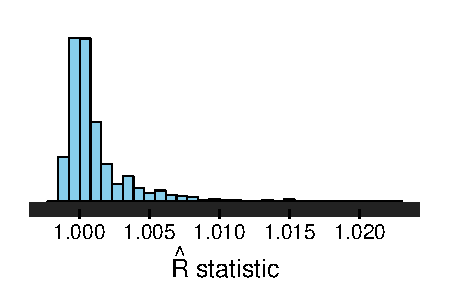
\includegraphics[scale=0.7]{sections/figs/rhat}
	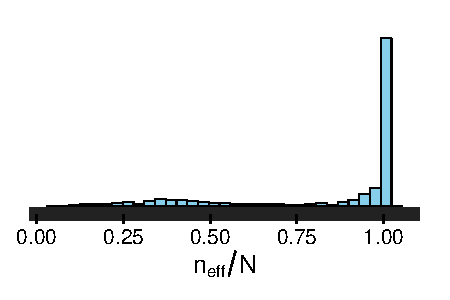
\includegraphics[scale=0.7]{sections/figs/neff}
	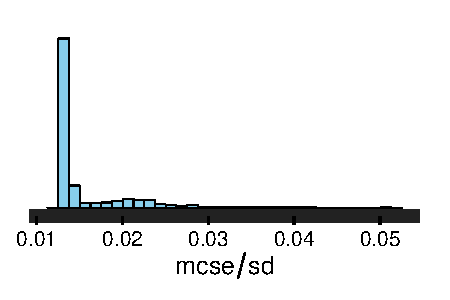
\includegraphics[scale=0.7]{sections/figs/mcse}
\caption{Distributions of diagnostics computed from the MCMC draws. 
From left to right: \newline ({\bf a}) Potential scale reduction factor $\hat{R}$ \newline ({\bf b}) 
Ratio of effective sample size to total sample size ($n_{\it eff}/N$) \newline ({\bf c}) Ratio of 
Monte Carlo error to posterior standard deviation ($mcse/sd$)}
\label{fig:ck_diagnostics}
\end{figure}

Panel ({\bf b}) shows the distribution of the ratio of effective sample size to the number of 
iterations ($n_{\it eff}/N$). Roughly speaking, $n_{\it eff}$ is an estimate of the number of 
{\it independent} draws from the posterior distribution that would have the same expected 
variance as the $N$ {\it dependent} draws actually obtained from the 
Markov chains. In the absence of autocorrelation $n_{\it eff} = N$, and so the ideal value of the ratio is one. 
In this case $n_{\it eff}/N$ is sufficiently large -- it is at least 20\% for all parameters -- and 
for most parameters the ratio is close to one, a reflection of Stan's efficiency. 


The distribution of the ratio of Monte Carlo error to the estimated standard 
deviation ($mcse/sd$) is shown in panel ({\bf c}) of Figure~\ref{fig:ck_diagnostics}. 
Monte Carlo error is a measure of imprecision due to approximating 
the posterior distribution by the MCMC simulations. As the number of iterations increases 
$mcse$ tends toward zero and the standard deviation of the draws converges to the posterior 
standard deviation. In this case, for all parameters the relative error $mcse/sd$ is less 
than five percent, which, for the inferential goals of this analysis, is negligible. 

For example, Figure~\ref{fig:ck_example_posterior} shows the estimated 
posterior density for the parameter corresponding to bias towards the majority party in the 79th 
congress.\footnote{There is nothing special about the 79th congress for this purpose. A single 
congress was chosen at random to use as an example.} The posterior is approximately Gaussian, 
with mean and standard deviation of roughly $0.054$ and $0.037$, respectively. The 
estimated $mcse$ is $0.0007$, which is inconsequential when compared to the uncertainty about 
the parameter in the posterior distribution.   


\begin{figure}[h]
\centering
	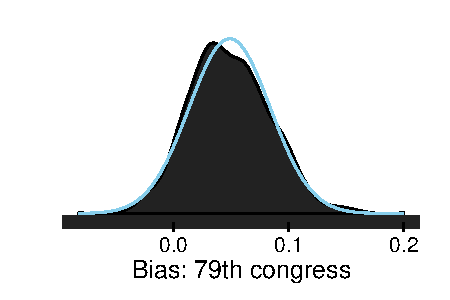
\includegraphics[scale=0.75]{sections/figs/example_posterior}
\caption{Posterior kernel density estimate for bias towards the majority party in the 79th congress. 
Normal density curve in blue.}
\label{fig:ck_example_posterior}
\end{figure}


%DEPENDENCE PLOT?
%
%
%\begin{figure}[h]
%\centering
%	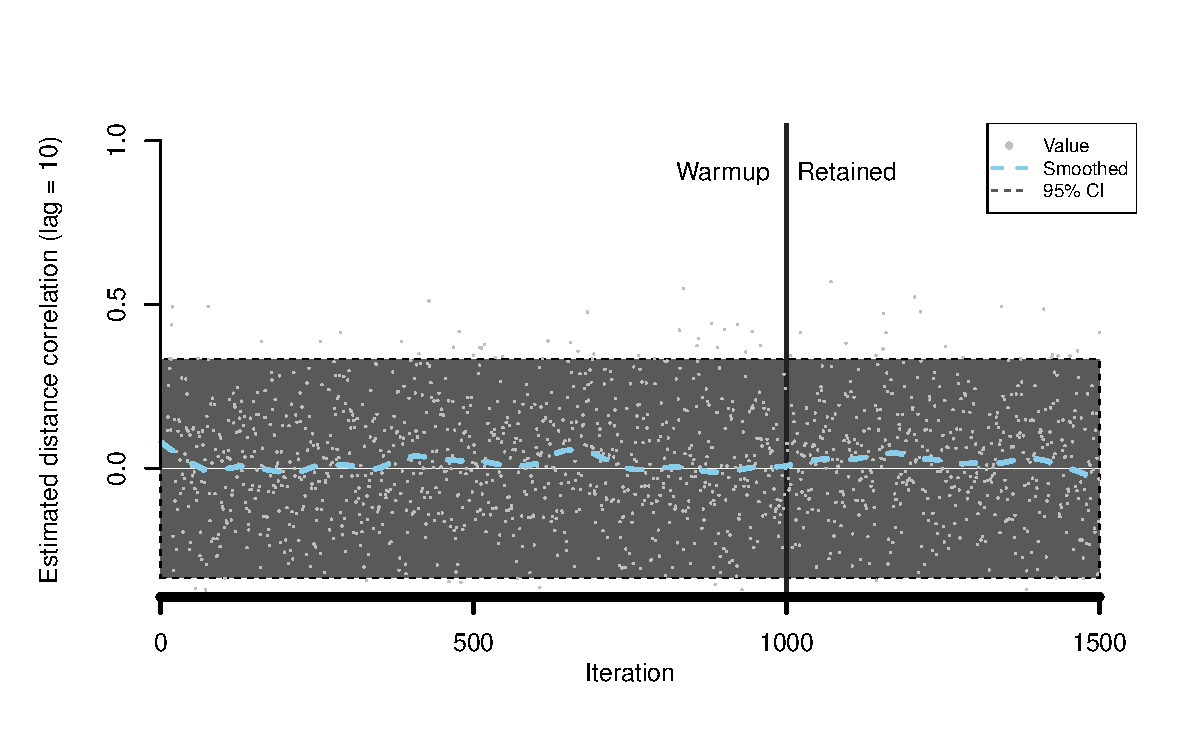
\includegraphics[scale=0.75]{sections/figs/ck_dependence}
%\caption{Estimated distance correlation among the eight chains. At a lag of 10 the draws are essentially independent. }
%\label{fig:ck_dependence}
%\end{figure}
%

In addition to the diagnostics discussed above, trace plots for all parameters were also 
examined as well as additional quantities specific to HMC and NUTS.\footnote{For example, 
checking that the tree depth used by NUTS is well below the user-specified maximum, ensuring 
that there are no post-warmup leapfrog iterations with diverging error, etc. These are explained 
in greater detail in \citeA{stan_development_team_stan_2015}.} 
Also see Appendix E (p.~\pageref{AppendixE}) % Appendix~\ref{AppendixF} 
for graphical posterior predictive model checking. 


\subsection[Estimates and discussion]{Estimated bias toward the majority party}
\label{results}

\subsubsection{Comparing the results}

Figure~\ref{fig:ck_bias} (p.~\pageref{fig:ck_bias}) juxtaposes the estimates of 
bias towards the majority party over time from Cox and Katz's analysis and the reanalysis 
using the Bayesian STAR model.

\begin{figure}
\centering
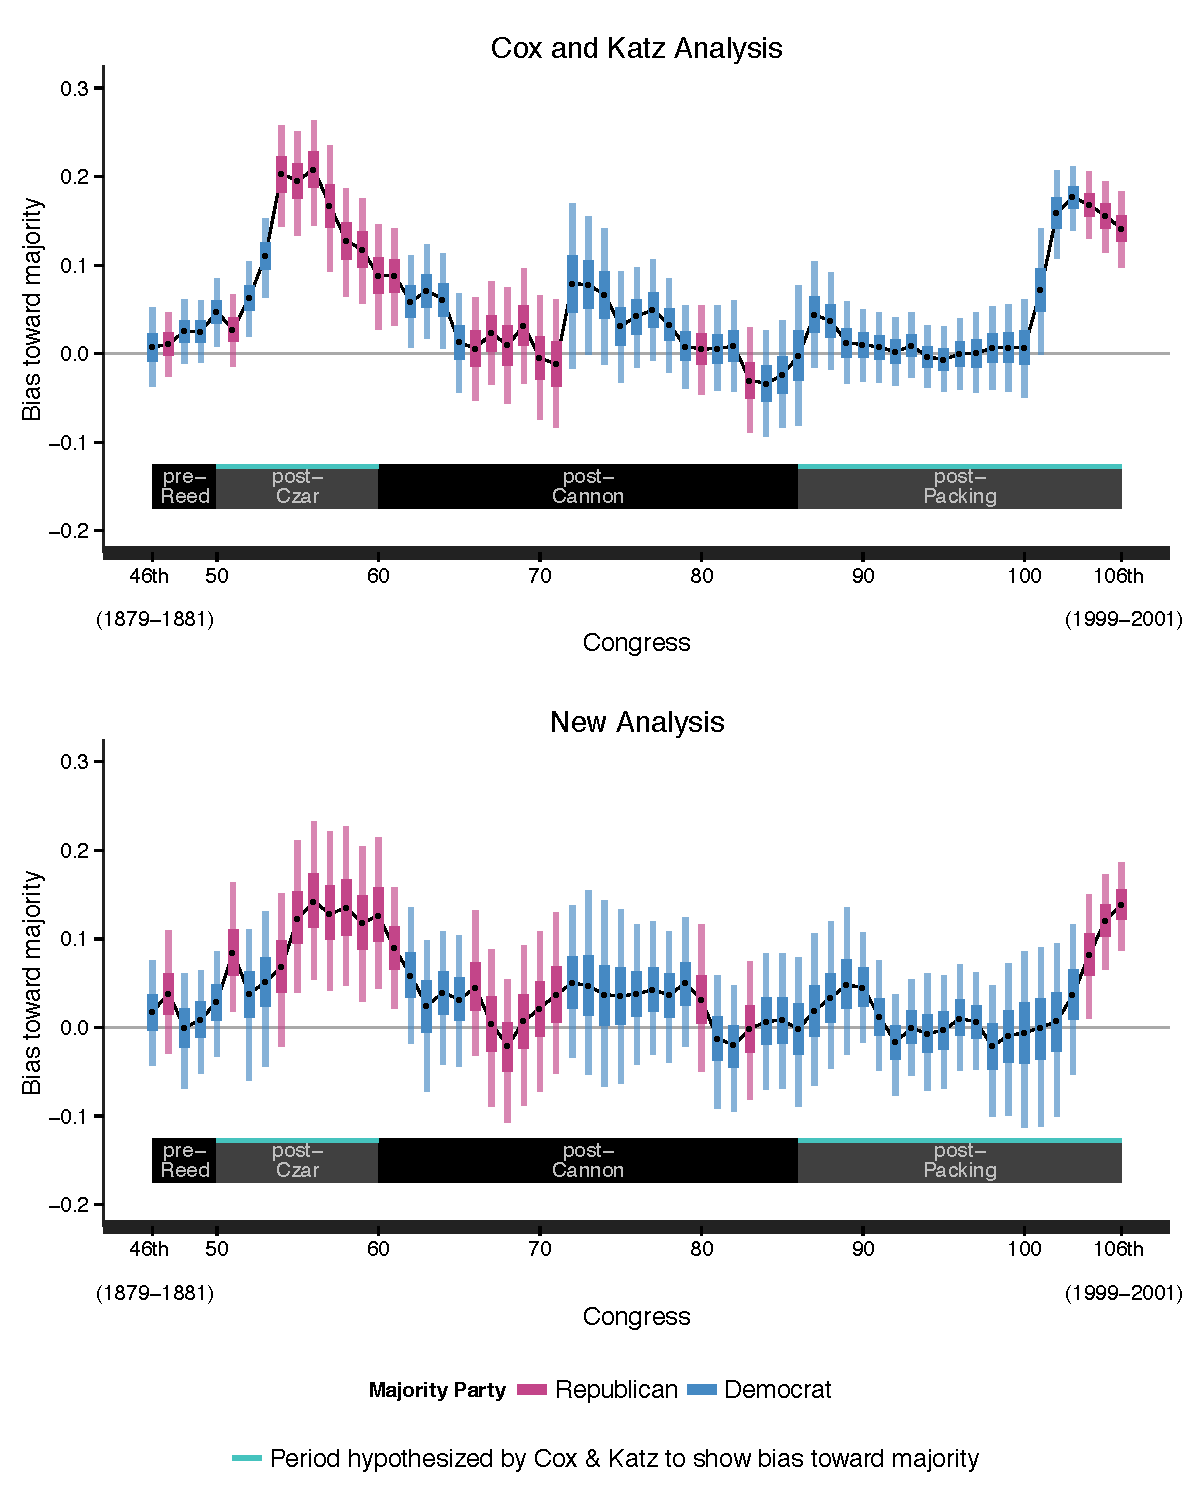
\includegraphics[scale=0.75]{sections/figs/ck_replication_new}
\caption{Estimated bias toward the majority party by Congress in 
Cox and Katz's analysis (top) and the Bayesian reanalysis (bottom). 
The thin and thick vertical segments represent 95\%  and 50\%
intervals, respectively.  The black line connects medians.
To produce the graph on top Cox and Katz's original analysis was 
replicated (see Figure 3 in Cox and Katz (2007)).}
\label{fig:ck_bias}
\end{figure}

Immediately noticeable is that the new estimates have greater 
uncertainties, which is to be expected due to the potential for Cox and Katz's method to 
produce overly precise estimates  (see section \ref{subsection_methods}). The new results 
do provide some support for the hypothesis of bias during the post-czar and post-packing 
periods; the evidence is much weaker than that found by Cox and Katz, but the finding 
of bias toward the Republican majority in the latter half of the post-czar period holds up. 

When compared to Cox and Katz's results, the hierarchical Bayesian STAR model estimates 
a more believable trend in bias over time. This can be seen clearly by comparing the curves 
in Figure~\ref{fig:ck_bias}. The smoothing prior shrinks each individual estimate slightly 
towards its neighbors -- the amount of smoothing is related to the hierarchical variance 
hyperparameter -- and all estimates are shrunk to the common prior mean, which helps 
avoid overfitting but still allows for substantial movement between Congresses 
if strongly supported by the data. Although both sets of results agree on the direction of 
bias in the post-czar period, while the Cox and Katz estimates show signs of overfitting 
the new estimates are less volatile. 


\subsubsection{Different interpretations}

Cox and Katz proceed with inference by comparing the statistical significance of their 
estimates. For example, they write ``In the pre-Reed era, the running average 
bias is statistically insignificant in four out of five Congresses \dots", and ``In the czar-rule era, 
the running average bias is statistically significant in nine out of ten Congresses \dots" 
\shortcite[p. 116]{cox_gerrymandering_2007}. This is problematic for several reasons.
First, if the reported standard errors understate the uncertainty in their estimates 
-- and this is presumably the case, as emphasized above and in \ref{subsection_methods} 
-- then they will be more likely to find statistical significance than is justified from the data, 
regardless of the arbitrary threshold selected for determining significance. Second, there
are numerous cases in which the difference between statistically significant bias in Congress 
$t$ and nonsignificant bias in Congress $t + 1$ (or vice-versa) is not itself statistically significant. 

Three such examples are given in Figure~\ref{fig:ck_signif}. The plot on the left, for instance, 
shows Cox and Katz's point estimates and 95\% intervals for bias in the 100th and 101st 
Congresses. The estimates (plus or minus one standard error) are $b_{100} = 0.0065 \pm 0.029$ 
and $b_{101} = 0.071 \pm 0.034$. Assuming the 95\% threshold for statistical significance 
standard in the social sciences and used by Cox and Katz, $b_{101}$ is statistically significant 
but $b_{100}$ is not. Though it is then tempting to conclude that one is signal while the other 
is indistinguishable from noise, note that the difference between the two is 
$0.0645$ with a standard error of $0.045$ and thus not close to statistically significant. 
The general point is counter-intuitive: nonsignificant changes can correspond to large shifts 
in significance levels.\footnote{A more detailed explanation of this issue -- which is not unique to this 
example -- and its potential consequences can be found in Chapter 2 of 
\citeA{gelman_arm_2007}.} When viewed from this perspective it is clear that comparisons of 
time periods based on the proportion of statistically significant estimates is not appropriate. 

\begin{figure}
\centering
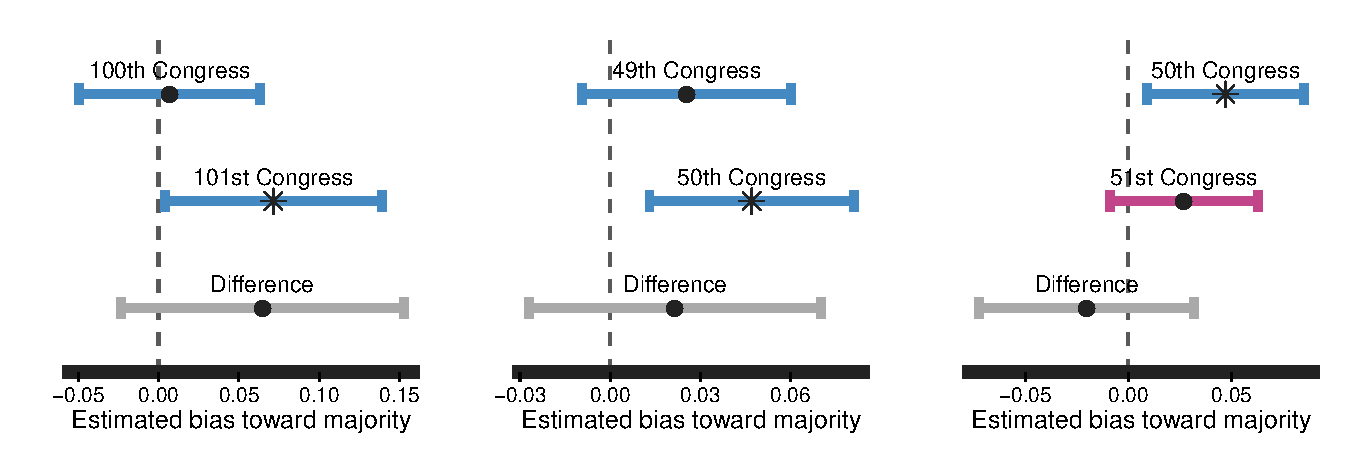
\includegraphics[scale=0.75]{sections/figs/ck_signif_all}%
%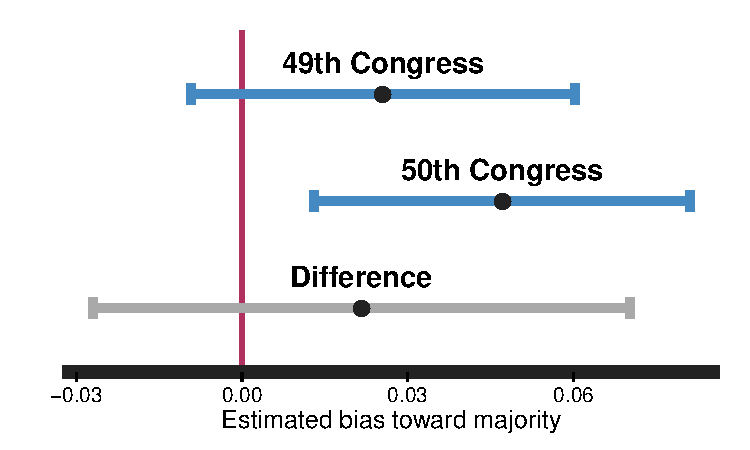
\includegraphics[scale=0.5]{sections/figs/ck_signif2}
\caption{Examples from Cox and Katz's results for which the difference between statistically 
significant and nonsignificant is not itself statistically significant.}
\label{fig:ck_signif}
\end{figure}

Cox and Katz's point estimates and confidence intervals obtained by maximum likelihood estimation 
are difficult to interpret for other reasons as well. The classical approach assesses each point estimate 
in relation to infinitely many potential intervals computed from infinitely many potential samples. But for 
an individual interval, what can be said is that it either contains the (abstract) true parameter value or it 
does not. This is a consequence of accepting (explicitly or implicitly) the classical position that the parameter 
is fixed but the data and interval bounds are random variables. 

On the contrary, from the Bayesian perspective the parameter is treated as a random 
variable while the data and intervals are fixed. As a consequence, results have a natural 
interpretation in terms of probabilities about the values of unknown parameters. 
The full Bayesian model provides an estimate of the marginal posterior {\it distribution} 
for each parameter. That is, the estimates are the distributions themselves, each of which 
represents an approximation of our a posteriori uncertainty about a certain parameter. 
Any so-called credible intervals computed from the posterior distribution have a more 
intuitive interpretation: the probability that the true parameter value lies in the $p\%$ interval  
-- conditional on the model and data -- is $p$. 

 


\subsubsection{Moving beyond Cox and Katz's rolling average approach}

As discussed in \ref{subsection_methods}, Cox and Katz's results comprise estimates taken 
from 61 separate models (one for each Congress). This results in the data for each Congress 
$t$ being reused in up to six of the 60 models besides the model for Congress $t$ itself. It also 
entails the exclusion of all data from Congresses outside each window. Furthermore, the decision
to use rolling windows of seven Congresses ($t \pm 3$) is arbitrary and difficult to subject to validity 
checks -- the assumptions of standard model comparison techniques are violated when each 
model to be compared is already itself an ad-hoc summary of many individual models (each
of which is estimated from a different subset of the data). 

\begin{figure}
\centering
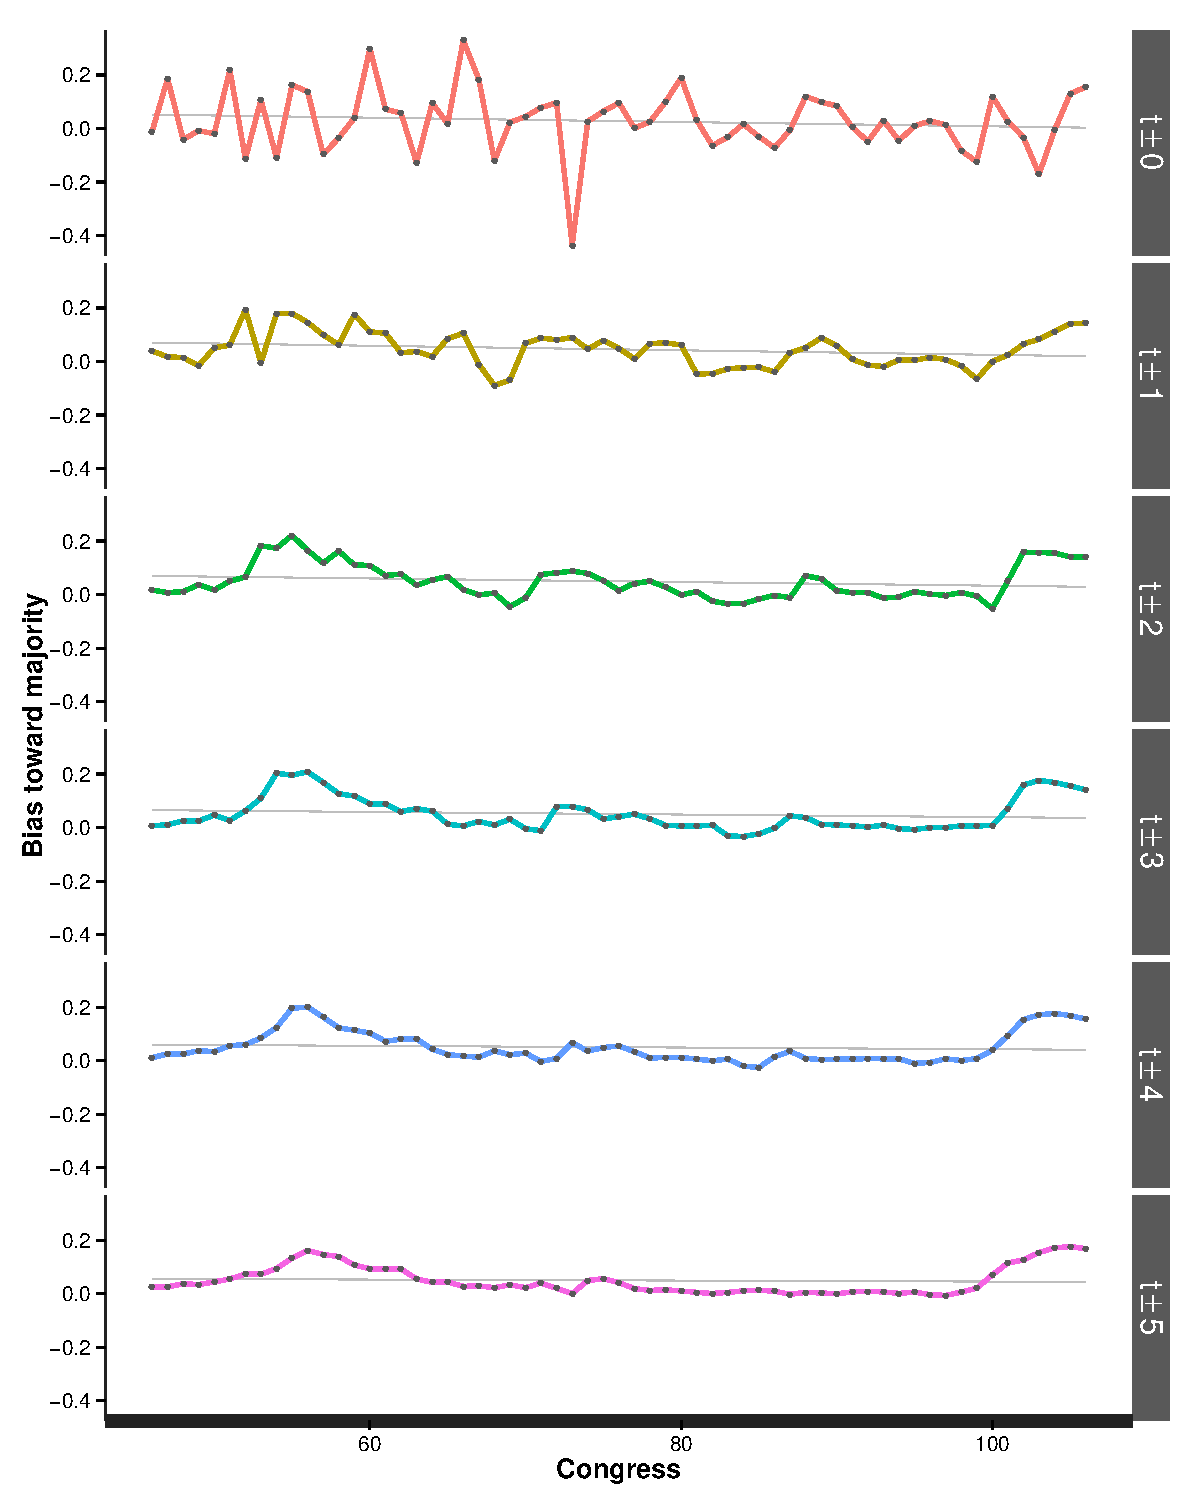
\includegraphics[scale=0.75]{sections/figs/ck_hypothetical}
\caption{Replications of Cox and Katz's results but changing the number of Congresses 
included when estimating each point. The top panel corresponds to estimating bias in each 
Congress $t$ using only data from time $t$ (i.e., $t \pm 0$). In each subsequent panel the 
set of Congresses is expanded by one in both directions. The bottom panel corresponds to 
using $t \pm 5$. The analysis presented in \protect\citeA{cox_gerrymandering_2007} is the 
panel for $t \pm 3$. The horizontal gray lines are the estimates obtained by completely 
pooling the data from all Congresses. Error bars are excluded so that differences in the 
smoothness of the curves are more perceptible.}
\label{fig:ck_hypothetical}
\end{figure}


The curves in Figure~\ref{fig:ck_hypothetical} (p.~\pageref{fig:ck_hypothetical}) show the 
results Cox and Katz would have found had they chosen narrower or wider windows. As the 
set of Congresses included in each model grows, the resulting curve necessarily becomes 
smoother because Cox and Katz's method is less and less distinguishable from simply 
estimating a common bias parameter for all Congresses (that is, assuming no variation in 
bias over time). Conversely, the single Bayesian model -- via the smoothness priors and  
hierarchical structure -- allows for bias in each Congress to depend on neighboring 
Congresses while using the entire dataset only once, obviating the need to dubiously subset 
the data. It also allows for comparing the fit of the model to other possible models (e.g., 
the $RW_2$ or other smoothness priors), something that will be explored in future work. 

\chapter{Discussion}
\label{discussion}

\section{Future directions}

For the reanalysis of \citeA{cox_gerrymandering_2007}, the hierarchical Bayesian model with first order 
undirected random walk priors is a promising start. In other work, we are exploring the sensitivity of the 
results to different possible smoothness priors including second order random walks (see \ref{reanalysis}), 
Gaussian process priors, and others. This will enable model comparisons that can 
illuminate the unique properties of the different approaches. We are also researching 
how the principles espoused by \citeA{wawro_designing_2014} can be woven into other statistical 
methods (from duration models to the detection of path dependence) and applied to diverse areas
of scholarship like democratic peace theory and studies of economic inequality. 
 

\section{Conclusion}

A statistical model is simpler than the reality it seeks to describe. In addition, the 
process of distilling the features of some phenomena into relationships concisely 
described by probability theory inevitably introduces error. A statistical model is 
therefore both a reduction and expansion of reality. For this reason, a social scientific 
application of statistical modeling is vacant in the absence of thoughtful qualitative 
work to endow the model with its meaningful information content. Successful 
applications are motivated by theory and supported by qualitative foundations. 

Following \citeA{wawro_designing_2014}, this thesis describes and demonstrates 
an alternative to the standard statistical methods adopted for the study of historical 
political institutions and, more broadly, historical social scientific inquiry. The new perspective is 
motivated by the criticism from qualitatively-inclined scholars of history that traditional methods 
are unsuited for capturing essential qualitative features of history. 
Wawro and Katznelson argue that failure to embrace more thoughtful, nuanced quantitative 
approaches will only reinforce the existing divisions between qualitative and quantitative 
researchers who otherwise share common aims. 

The reanalysis of \citeA{cox_gerrymandering_2007}
provides another case study -- in addition to the analyses conducted by Katznelson and 
Wawro -- showing how hierarchical models with smoothness priors can better incorporate 
context and temporality into a quantitative historical analysis. These models are 
natural to construct in a Bayesian framework, accommodate greater parameter variation, 
and allow periodization schemes be substantially data-dependent.  
Stan provides a flexible language for expressing these models and 
enables full Bayesian inference to be carried out more efficiently than 
previously possible.  

While successful quantitative analysis has a qualitative backbone, 
the converse is often not true. The historical social scientific literature 
is rife with theories lacking corroboration (or opposition) in the form of rigorous 
data analysis. In isolation, quantitative methods are hollow and
qualitative methods are insufficient. Their union offers the potential for 
the richest scholarship. As the inventory of promising applications of Wawro and 
Katznelson's proposals grows, hopefully historians and qualitatively-oriented 
scholars will embrace the progress in quantitative analysis and provide informed 
critiques supported by statistical theory. 


%\chapter{Farhang and Katznelson}

To illustrate the utility of STAR models, Wawro and Katznelson (2013) conduct a reanalysis of Farhang and Katznelson (2005). Farhang and Katznelson argue that drastic changes in the Democratic party's position on labor-friendly policies occurred during the time period of time between New Deal and Fair Deal, largely due to a growing divide between norther and southern Democrats. 

In this section we expand on the reanalysis proposed by Wawro and Katznelson. 

% Something about how this analysis includes time and space as opposed to cox and katz which is just time

\section{Data} 

The data used by Farhang and Katznelson pertains to roll-call votes in the 73rd through 80th Congresses (1933--1948). The outcome of interest is a binary variable indicating whether a senator $s$ from region $r$ voted in favor of the prolabor position on roll-call vote $v$ in Congress $t$

$$L_{srtv} = 
\begin{cases}
1, & \text{ if senator $s$ from region $r$ votes prolabor on vote $v$ at time $t$} \\
0, & \text{ otherwise.}
\end{cases}
$$

The possible values for region are Non-South (NS), Border South (BS), and Deep South (DS). 

Predictors include the proportion of African Americans living in the senator's home region $(AA)$, the proportion of individual's in the senator's home region living in urban areas ($URB$), a measure of unionization 
%\footnote{Include description from W\&K paper}
$(UN)$, and indicators for Democratic party membership $(DEM)$ and membership on the committee charged with overseeing labor-related issues $(COM)$.  % this is maybe too close to the wording in W&K

% say something about why these variables are relevant

% FIGURES summarizing data % 

\section{Method of analysis}

\subsection{The map as an undirected graph}

Unlike in the Cox and Katz analysis, here we want to account for variation and dependence over both temporal and spatial dimensions. From the three regions and eight congresses in the data we construct the $3 \times 8$ map with cells $c_1,c_2, \dots, c_{24}$ shown in Table~\ref{table:map_degree}. The value displayed in cell $c_{j}$ is the number of cells considered neighbors of $c_{j}$

$$ c_{j} = \sum_{k = 1}^{24} \textit{Ne}(j,k),$$

\noindent where the neighbor function $\textit{Ne}(j,k)$ is 1 if $c_j$ and $c_k$ are neighbors and $0$ otherwise. The value of each $c_j$ is determined by our subjective choice of the form of the neighbor function, which should be informed by a substantive theory about the temporal and spatial dependence. 

The values in Table~\ref{table:map_degree} correspond to using an undirected neighbor function that considers adjacency to be vertical, horizontal and diagonal. For example, this form of the neighbor function allows for dependence between the Border South region in the 76th Congress and the Non-South region in the 77th Congress. Other possible neighbor functions might only allow for dependence across regions in the same time period, or only allow dependence on prior time periods, or allow dependence on time periods even further into the past or future.    

%\begin{table}[ht]
%\centering
%\begin{tabular}{l|rrrrrrrr}
%\textbf{Region}/\textbf{Congress} & 73rd & 74th & 75th & 76th & 77th & 78th & 79th & 80th \\ 
%  \toprule
%Non-South &   1 &   4 &   7 &  10 &  13 &  16 &  19 &  22 \\ 
%  Border South &   2 &   5 &   8 &  11 &  14 &  17 &  20 &  23 \\ 
%  Deep South &   3 &   6 &   9 &  12 &  15 &  18 &  21 &  24 \\ 
%   \bottomrule
%\end{tabular}
%\caption{\small The $3 \times 8$ map assigning a unique identifier for each region/Congress pair}
%\label{table:map_id}
%\end{table}


\begin{table}[ht]
\centering
\begin{tabular}{l|rrrrrrrr}
\textbf{Region}/\textbf{Congress} & 73rd & 74th & 75th & 76th & 77th & 78th & 79th & 80th \\ 
 \toprule
Non-South 	
& $3_{(1)}$ & $5_{(4)}$ & $5_{(7)}$ & $5_{(10)}$ & $5_{(13)}$ & $5_{(16)}$ & $5_{(19)}$ & $3_{(22)}$ \\ 
Border South 	
& $5_{(2)}$ & $8_{(5)}$ & $8_{(8)}$ & $8_{(11)}$ & $8_{(14)}$ & $8_{(17)}$ & $8_{(20)}$ & $5_{(23)}$ \\ 
Deep South 	
& $3_{(3)}$ & $5_{(6)}$ & $5_{(9)}$ & $5_{(12)}$ & $5_{(15)}$ & $5_{(18)}$ & $5_{(21)}$ & $3_{(24)}$ \\ 
   \bottomrule
\end{tabular}
\caption{\small The $3 \times 8$ map where the cell contents are the number of neighbors. The subscripts assign each region/Congress pair a unique identifier from 1 to 24. Adjacency is vertical, horizontal, and diagonal.}
\label{table:map_degree}
\end{table}


Using the indices $r \in \{1,\dots, R\}$ (where in this case $R = 24$) from Table~\ref{table:map_degree}, we can 
reconceptualize the map as an undirected graph with $R$ vertices and with edges connecting neighbors. We can then make the two $R \times R$ matrices -- the symmetric adjacency matrix and diagonal degree matrix -- needed for constructing the precision matrix for the GMRF prior. 


%\clearpage
%
%\subsection{Notation}
%
%\begin{tabular}{ll}
%$N \approx 8000$ & Number of observations in the data. \\[5pt]
%
%$R = 24$ & Number of groups (i.e. region/period combos).  \\[5pt]
%
%$\textsc{urb}$, $\textsc{aa}$, $\textsc{un}$ & The three $N \times 1$ vectors for {\tt urbanpct}, {\tt aapct}, and {\tt unionpop} variables. \\[5pt]
%
%$\mathbf{M}$ & $N \times R$ matrix with $m_{ij} = 1$ if obs $i$ is from region-period $j$, and 0 otherwise. \\[5pt]
%
%$\mathbf{X}_1, \mathbf{X}_2, \mathbf{X}_3$ & $N \times R$ matrices with $x_{ij} =$ $i$th value of 
% \textsc{urb} (for $\mathbf{X}_1$), \textsc{aa} (for $\mathbf{X}_2$), \\
% 
% & or \textsc{un} (for $\mathbf{X}_3$) if obs $i$ is from region-period $j$, and 0 otherwise. \\[5pt]
%
%$\mathbf{Z} $ & $N \times 2$ matrix with party and committee indicators.  \\[5pt]
%
%$y$ & $N \times 1$ vector containing the indicator for pro-labor vote. 
%
%\end{tabular}



\vskip1in
\subsection{Model}

Conditional on parameters $\theta$, the observations of the binary indicator $L$ are assumed to be independent and follow a Bernoulli distribution. Here, the structured additive predictor $\eta = {\rm logit}(\theta)$ is 

$$\log{\left(\frac{\theta_{srtv}}{1 - \theta_{srtv}}\right)} = \eta_{srvt} = \alpha_0 + f_1 (\alpha_{rt}) + f_2 (UN_{srt}) + f_3 (URB_{srt}) + f4(AA_{srt}) + u_{srt}' \gamma, $$

\noindent where $\alpha_0$ represents a global intercept, $\alpha_{rt}$ is the region-period specific deviation from $\alpha_0$, and $\mathbf{u}$ includes $DEM$ and $COM$, predictors with effects assumed not to vary across region and time period.
 
As in the Cox and Katz model, we can express the vector of evaluations of each unknown function $f_j$ as the product of a design matrix $\mathbf{M}_j$ and a parameter vector, here denoted $\beta_j$. We can then write the structured additive predictor $\eta$ in matrix form as 
 
$$\eta = \mathbf{u}\gamma + \alpha_0 + \left( \sum_{j=1}^{4} \mathbf{M}_j \beta_j \right). $$
 
Specifying GMRF smoothness priors over regions and periods corresponds to the zero-mean multivariate normal priors

$$ p(\beta_j | \tau^2_j) \propto  \exp{\left(-\frac{1}{2\tau_j^2} \beta_j^T \mathbf{P}^{-1} \beta_j \right)}. $$

Weakly informative Gaussian priors are used for the coefficients $\gamma$. Prior distributions for the global intercept $\alpha_0$ and the hyperparameters $\tau_j$ are discussed below in the Estimation section. 








%For $j = 1, \dots, J$ the precision matrix $\mathbf{K}_j$ is defined as $\mathbf{K}_j = \tau_j \left(\mathbf{D} - \rho_j \mathbf{A}\right).$ The matrices $\mathbf{A}$ and $\mathbf{D}$ are the symmetric adjacency matrix and diagonal degree matrix. 
%
%\vskip 1cm
%
%For each precision matrix $\mathbf{K}_{R \times R}$, we can interpret its elements as follows:
%
%\begin{itemize}
%\item For $i \neq j$, element $k_{ij}$ is conditional covariance between $i$ and $j$, given all the variables except $i$ and $j$, except the sign of the conditional covariance is flipped.
%
%\item For $i = j$, element $K_{ij}$ is the conditional variance of $i$, given all the variables except $i$.
%\end{itemize}
%
%This enables us to go from the full-conditional relationships that GeoBUGS utilizes for Gibbs sampling to the joint form that Stan needs for HMC. \\
%
%


%\subsection{Hyperpriors}
%
%Let $\lambda_j \sim {\rm Exponential}(1)$ and let $\tau_j = \bar{\tau}\lambda_j $, which implies
%
%$$\tau_j \sim {\rm Exponential}(1/\bar{\tau}), $$
%
%where $\bar{\tau} > 0$ is the common mean for the $\tau_j$'s. Give $\bar{\tau}$ an improper flat prior over $\mathbb{R}^+.$ \\
%
%
%
%
%\noindent Let $\rho_j \sim {\rm Beta}(s_1, s_2)$, where $s_1 = \gamma \bar{\rho}$,  and $s_2 = \gamma(1-\bar{\rho})$, where $\gamma$ is either an estimated positive dispersion parameter or fixed (e.g. $\gamma = 1$). For the common mean $\bar{\rho} \in (0,1)$ let $\bar{\rho} \sim {\rm Unif}(0,1)$.    \\







%
%\begin{table}[ht]
%\scriptsize
%\centering
%$$  \begin{array}{r|rrrrrrrrrrrrrrrrrrrrrrrr} 
%  & 1 & 2 & 3 & 4 & 5 & 6 & 7 & 8 & 9 & 10 & 11 & 12 & 13 & 14 & 15 & 16 & 17 & 18 & 19 & 20 & 21 & 22 & 23 & 24 \\ 
%\midrule
%1 & 3 & \!-1\! & 0 & \!-1\! & \!-1\! & 0 & 0 & 0 & 0 & 0 & 0 & 0 & 0 & 0 & 0 & 0 & 0 & 0 & 0 & 0 & 0 & 0 & 0 & 0 \\ 
%  2 & \!-1\! & 5 & \!-1\! & \!-1\! & \!-1\! & \!-1\! & 0 & 0 & 0 & 0 & 0 & 0 & 0 & 0 & 0 & 0 & 0 & 0 & 0 & 0 & 0 & 0 & 0 & 0 \\ 
%  3 & 0 & \!-1\! & 3 & 0 & \!-1\! & \!-1\! & 0 & 0 & 0 & 0 & 0 & 0 & 0 & 0 & 0 & 0 & 0 & 0 & 0 & 0 & 0 & 0 & 0 & 0 \\ 
%  4 & \!-1\! & \!-1\! & 0 & 5 & \!-1\! & 0 & \!-1\! & \!-1\! & 0 & 0 & 0 & 0 & 0 & 0 & 0 & 0 & 0 & 0 & 0 & 0 & 0 & 0 & 0 & 0 \\ 
%  5 & \!-1\! & \!-1\! & \!-1\! & \!-1\! & 8 & \!-1\! & \!-1\! & \!-1\! & \!-1\! & 0 & 0 & 0 & 0 & 0 & 0 & 0 & 0 & 0 & 0 & 0 & 0 & 0 & 0 & 0 \\ 
%  6 & 0 & \!-1\! & \!-1\! & 0 & \!-1\! & 5 & 0 & \!-1\! & \!-1\! & 0 & 0 & 0 & 0 & 0 & 0 & 0 & 0 & 0 & 0 & 0 & 0 & 0 & 0 & 0 \\ 
%  7 & 0 & 0 & 0 & \!-1\! & \!-1\! & 0 & 5 & \!-1\! & 0 & \!-1\! & \!-1\! & 0 & 0 & 0 & 0 & 0 & 0 & 0 & 0 & 0 & 0 & 0 & 0 & 0 \\ 
%  8 & 0 & 0 & 0 & \!-1\! & \!-1\! & \!-1\! & \!-1\! & 8 & \!-1\! & \!-1\! & \!-1\! & \!-1\! & 0 & 0 & 0 & 0 & 0 & 0 & 0 & 0 & 0 & 0 & 0 & 0 \\ 
%  9 & 0 & 0 & 0 & 0 & \!-1\! & \!-1\! & 0 & \!-1\! & 5 & 0 & \!-1\! & \!-1\! & 0 & 0 & 0 & 0 & 0 & 0 & 0 & 0 & 0 & 0 & 0 & 0 \\ 
%  10 & 0 & 0 & 0 & 0 & 0 & 0 & \!-1\! & \!-1\! & 0 & 5 & \!-1\! & 0 & \!-1\! & \!-1\! & 0 & 0 & 0 & 0 & 0 & 0 & 0 & 0 & 0 & 0 \\ 
%  11 & 0 & 0 & 0 & 0 & 0 & 0 & \!-1\! & \!-1\! & \!-1\! & \!-1\! & 8 & \!-1\! & \!-1\! & \!-1\! & \!-1\! & 0 & 0 & 0 & 0 & 0 & 0 & 0 & 0 & 0 \\ 
%  12 & 0 & 0 & 0 & 0 & 0 & 0 & 0 & \!-1\! & \!-1\! & 0 & \!-1\! & 5 & 0 & \!-1\! & \!-1\! & 0 & 0 & 0 & 0 & 0 & 0 & 0 & 0 & 0 \\ 
%  13 & 0 & 0 & 0 & 0 & 0 & 0 & 0 & 0 & 0 & \!-1\! & \!-1\! & 0 & 5 & \!-1\! & 0 & \!-1\! & \!-1\! & 0 & 0 & 0 & 0 & 0 & 0 & 0 \\ 
%  14 & 0 & 0 & 0 & 0 & 0 & 0 & 0 & 0 & 0 & \!-1\! & \!-1\! & \!-1\! & \!-1\! & 8 & \!-1\! & \!-1\! & \!-1\! & \!-1\! & 0 & 0 & 0 & 0 & 0 & 0 \\ 
%  15 & 0 & 0 & 0 & 0 & 0 & 0 & 0 & 0 & 0 & 0 & \!-1\! & \!-1\! & 0 & \!-1\! & 5 & 0 & \!-1\! & \!-1\! & 0 & 0 & 0 & 0 & 0 & 0 \\ 
%  16 & 0 & 0 & 0 & 0 & 0 & 0 & 0 & 0 & 0 & 0 & 0 & 0 & \!-1\! & \!-1\! & 0 & 5 & \!-1\! & 0 & \!-1\! & \!-1\! & 0 & 0 & 0 & 0 \\ 
%  17 & 0 & 0 & 0 & 0 & 0 & 0 & 0 & 0 & 0 & 0 & 0 & 0 & \!-1\! & \!-1\! & \!-1\! & \!-1\! & 8 & \!-1\! & \!-1\! & \!-1\! & \!-1\! & 0 & 0 & 0 \\ 
%  18 & 0 & 0 & 0 & 0 & 0 & 0 & 0 & 0 & 0 & 0 & 0 & 0 & 0 & \!-1\! & \!-1\! & 0 & \!-1\! & 5 & 0 & \!-1\! & \!-1\! & 0 & 0 & 0 \\ 
%  19 & 0 & 0 & 0 & 0 & 0 & 0 & 0 & 0 & 0 & 0 & 0 & 0 & 0 & 0 & 0 & \!-1\! & \!-1\! & 0 & 5 & \!-1\! & 0 & \!-1\! & \!-1\! & 0 \\ 
%  20 & 0 & 0 & 0 & 0 & 0 & 0 & 0 & 0 & 0 & 0 & 0 & 0 & 0 & 0 & 0 & \!-1\! & \!-1\! & \!-1\! & \!-1\! & 8 & \!-1\! & \!-1\! & \!-1\! & \!-1\! \\ 
%  21 & 0 & 0 & 0 & 0 & 0 & 0 & 0 & 0 & 0 & 0 & 0 & 0 & 0 & 0 & 0 & 0 & \!-1\! & \!-1\! & 0 & \!-1\! & 5 & 0 & \!-1\! & \!-1\! \\ 
%  22 & 0 & 0 & 0 & 0 & 0 & 0 & 0 & 0 & 0 & 0 & 0 & 0 & 0 & 0 & 0 & 0 & 0 & 0 & \!-1\! & \!-1\! & 0 & 3 & \!-1\! & 0 \\ 
%  23 & 0 & 0 & 0 & 0 & 0 & 0 & 0 & 0 & 0 & 0 & 0 & 0 & 0 & 0 & 0 & 0 & 0 & 0 & \!-1\! & \!-1\! & \!-1\! & \!-1\! & 5 & \!-1\! \\ 
%  24 & 0 & 0 & 0 & 0 & 0 & 0 & 0 & 0 & 0 & 0 & 0 & 0 & 0 & 0 & 0 & 0 & 0 & 0 & 0 & \!-1\! & \!-1\! & 0 & \!-1\! & 3 \\ 
%\end{array} $$
%\caption{The ``Laplacian matrix" $\mathbf{L} = \mathbf{D} - \mathbf{A}$. The precision matrix $\mathbf{K}_j$ is $\mathbf{K}_j = \tau_j (\mathbf{D} - \rho_j \mathbf{A})$, where $\tau_j  > 0$ and $\rho_j \in (0,1)$. Thus $\rho_j \to 1 \implies \mathbf{K}_j \to \tau_j \mathbf{L}$.}
%\end{table}






\nocite{r_software}
\nocite{breslow_approximate_1993}



\begingroup
    \setstretch{1}
    \setlength\bibitemsep{1\baselineskip}
    \bibliography{bibliography.bib}
%     \addcontentsline{toc}{chapter}{References}
\endgroup


\begin{appendices}


\chapter{Impropriety of the GMRF prior} \label{AppendixA}

The penalty matrix $\mathbf{P}$ corresponding to an undirected $RW_\kappa$ prior over parameter vector $\lambda \in \mathbb{R}^C$ has rank $C - \kappa$ and the resulting matrix $\Sigma^{-1} = \mathbf{Q} = \mathbf{P}/\tau^2$ is not a valid precision matrix. In the $RW_1$ case this can be mitigated by jittering the elements of $\mathbf{P}$. For $\kappa > 1$ a possibility is to estimate only $C - \kappa$ of the $C$ parameters in $\lambda$,  from which the remaining $\kappa$ so-called {\it pinned} parameters (each of which has a conditional variance of zero) can be computed following the properties of the multivariate normal distribution. This strategy amounts to  constraining the relevant linear combinations to have zero variance, from which a proper prior on a lower dimensional subspace is obtained \shortcite{paciorek_2009, rue_gaussian_2005}. 

Another possibility is to estimate the autoregressive parameter $\omega$ mentioned in \ref{penalty_matrix} (see footnote~\ref{footnote_car}), which results in a proper prior. \citeA<See>{paciorek_2009} \citeA<and>{banerjee_hierarchical_2004} for potential drawbacks to this approach.

An entirely different tactic would be to estimate an arbitrary tridiagonal precision matrix rather than specifying the penalty matrix and estimating the hierarchical variance/precision parameter. One way to do this would be to decompose the precision matrix into conditional correlations and standard deviations. This is possible to do in Stan and should be explored in future work to sidestep the matrix singularity problems. 


\end{appendices}


\end{document}